\subsection{Version 1 vom UI-Konzept}

Hier sind die älteren Entwürfe des Designs. Bei diesen Entwürfen haben wir uns nur auf die Struktur
konzentriert und eine grobe Version erstellt. Uns war es hier hauptsächlich wichtig
die Ideen, die wir durch die Recherche aufgenommen haben zu projizieren.
\\
\newpage
\subsubsection{Version 1 Webchat}
Hier sieht man die älteren UI Designs Versionen, die zum Teil Chatfenster gehören.

\begin{figure}[H]
    \centering
    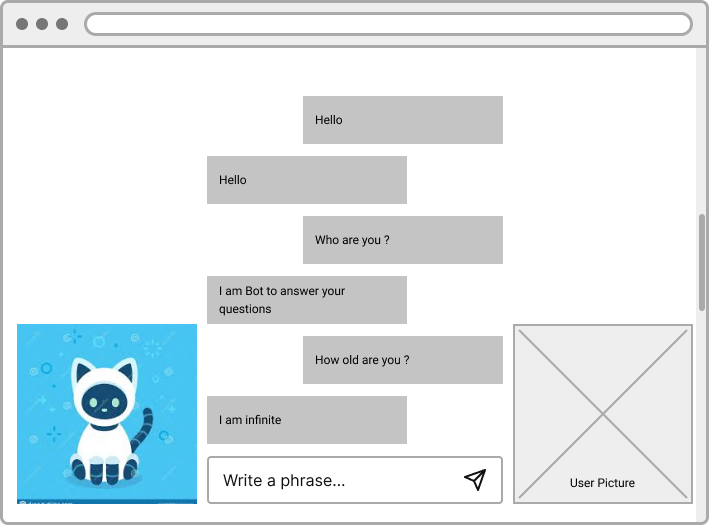
\includegraphics[width=0.8\textwidth]{bilder/old vers. UI Design/WebChat.png}
    \caption{Old version UI Design WebChat}
    \label{fig:Old version UI Design WebChat}
    \end{figure}
\noindent \textbf{Webchat} \newline
In der alten Version unseres Webchat Designs haben wir gedacht, auch für den
Nutzer ein Profilbild hinzuzufügen. Diese Idee schien aber zu aufwendig zu sein und wir versuchten
zuerst ein Minimal Viable Product zu erschaffen.                                                     

\newpage

\subsubsection{Version 1 Admin Interface Allgemein}
Hier sieht man die älteren UI Designs Versionen, die zum Teil Admin-Interface Allgemein gehören.

\begin{figure}[H]
    \centering
    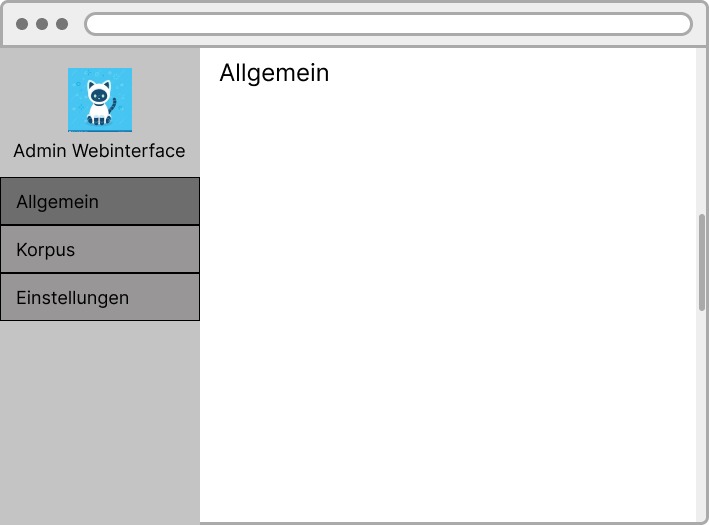
\includegraphics[width=0.8\textwidth]{bilder/old vers. UI Design/Admin Interface Allgemein.png}
    \caption{Old version UI Design Admin Interface Allgemein}
    \label{fig:Old version UI Design Admin Interface Allgemein}
    \end{figure}
\noindent \textbf{Admin Interface: Allgemein} \newline
Im Admin Interface kann man auf der linken Seite das Menü sehen. Was aber hier fehlt ist der Logout Button.
Wir hatten auch keine richtigen Vorstellungen, was wir einführen möchten.

\newpage

\subsubsection{Version 1 Admin Interface Korpus}
Hier sieht man die älteren UI Designs Versionen, die zum Teil Admin-Interface Korpus gehören.

\begin{figure}[H]
    \centering
    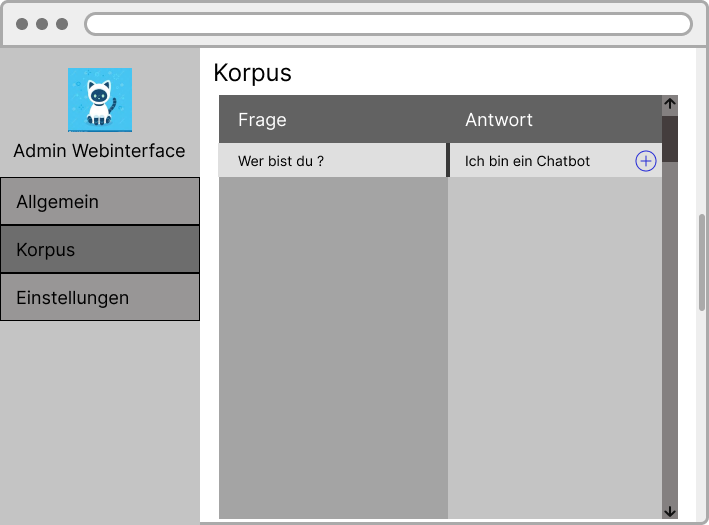
\includegraphics[width=0.8\textwidth]{bilder/old vers. UI Design/Admin Interface (1).png}
    \caption{Old version UI Design Admin Interface Korpus 00}
    \label{fig:Old version UI Design Admin Interface Korpus 00}
    \end{figure}
\noindent \textbf{Admin Interface: Korpus 00} \newline
Im Korpus wollten wir schon von Anfang an das Hinzufügen darstellen, wussten aber nicht
wie und haben herumprobiert.

\begin{figure}[H]
    \centering
    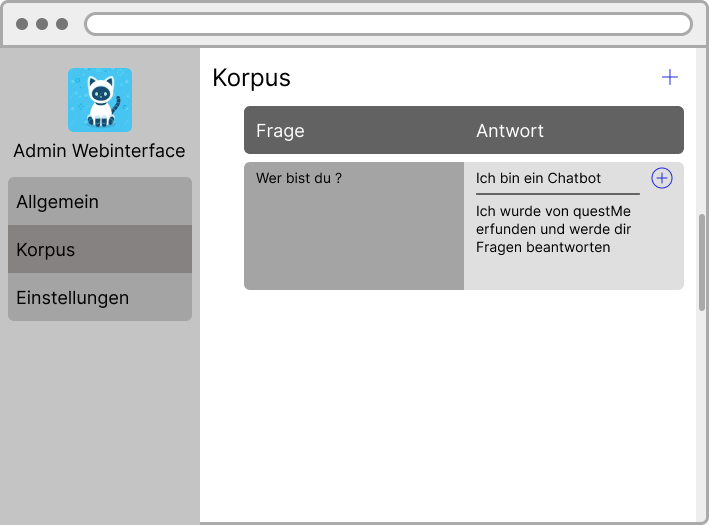
\includegraphics[width=0.8\textwidth]{bilder/old vers. UI Design/Admin Interface I.png}
    \caption{Old version UI Design Admin Interface Korpus 01}
    \label{fig:Old version UI Design Admin Interface Korpus 01}
    \end{figure}
\noindent \textbf{Admin Interface: Korpus 01} \newline
In diesem Beispiel sieht man ein Basisbeispiel mit einer Frage, die im Alltag gestellt wird und die dazugehörenden Antworten. Wie wir diese aber
editieren haben wir hier noch nicht gezeigt.

\begin{figure}[H]
    \centering
    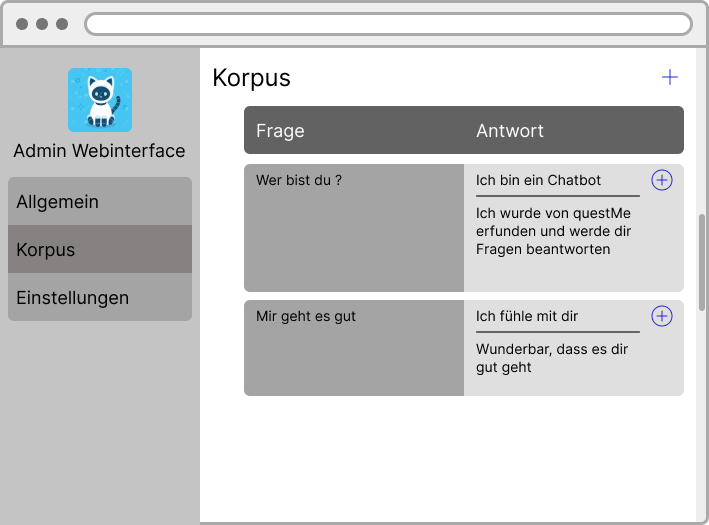
\includegraphics[width=0.8\textwidth]{bilder/old vers. UI Design/Admin Interface II.png}
    \caption{Old version UI Design Admin Interface Korpus 02}
    \label{fig:Old version UI Design Admin Interface Korpus 02}
    \end{figure}
\noindent \textbf{Admin Interface: Korpus 02} \newline
Im nächsten Beispiel sieht man eine weitere Frage und die dazugehörenden zwei Antworten. Es ist immer noch nicht
bekannt, wie man Antworten und Fragen editiert oder Fragen und Antworten von verschiedenen Domänen bearbeitet.

\newpage

\subsubsection{Version 1 Admin Interface Login}
Hier sieht man die älteren UI Designs Versionen, die zum Teil Admin-Interface Login gehören.

\begin{figure}[H]
    \centering
    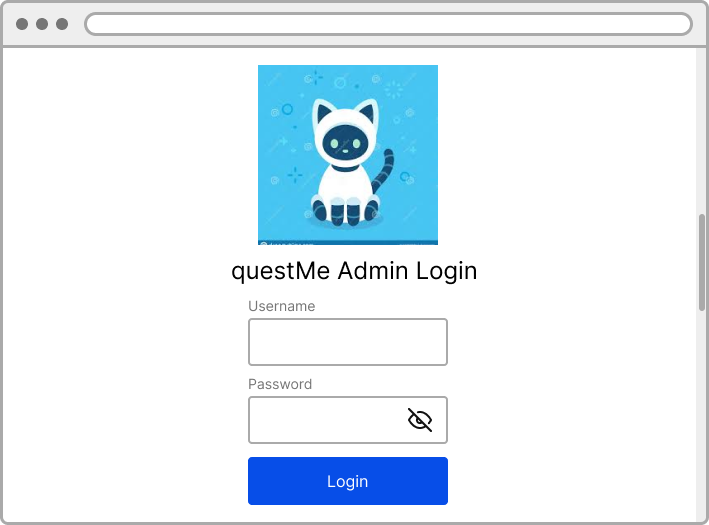
\includegraphics[width=0.8\textwidth]{bilder/old vers. UI Design/Admin Interface.png}
    \caption{Old version UI Design Admin Interface Login}
    \label{fig:Old version UI Design Admin Interface Login}
    \end{figure}
\noindent \textbf{Admin Interface: Admin Login} \newline
Hier haben wir nur ein klassisches Login Eingabefeld dargestellt, weil wir uns nicht klar waren, wie es mit der Authentifizierung und dem Admin
Login funktioniert.


\newpage

\subsection{Version 2 von UI-Konzept}
Hier sieht man die neuen Entwürfe des UI Designs. In der neuen Version werden auch die 
mobilen Versionen entworfen. Weil der Plan ist, zuerst eine mobile first Anwendung herzustellen.

\subsubsection{Version 2 Webchat}
Hier werden die neueren Versionen des UI Designs für den Webchat vorgestellt.
\begin{figure}[H]
    \centering
    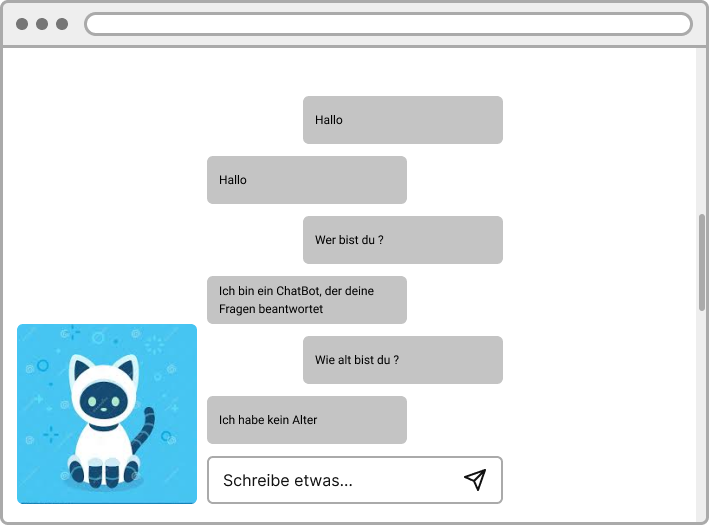
\includegraphics[width=0.8\textwidth]{bilder/new vers. UI Design/WebChat/WebChat.png}
    \caption{New version UI Design Webchat}
    \label{fig:New version UI Design Webchat}
    \end{figure}
\noindent \textbf{Webchat} \newline
Hier haben wir einen Beispielchat mit dem Bot dargestellt. In diesem Beispiel haben wir ein
Basisgespräch geführt.

\begin{figure}[H]
    \centering
    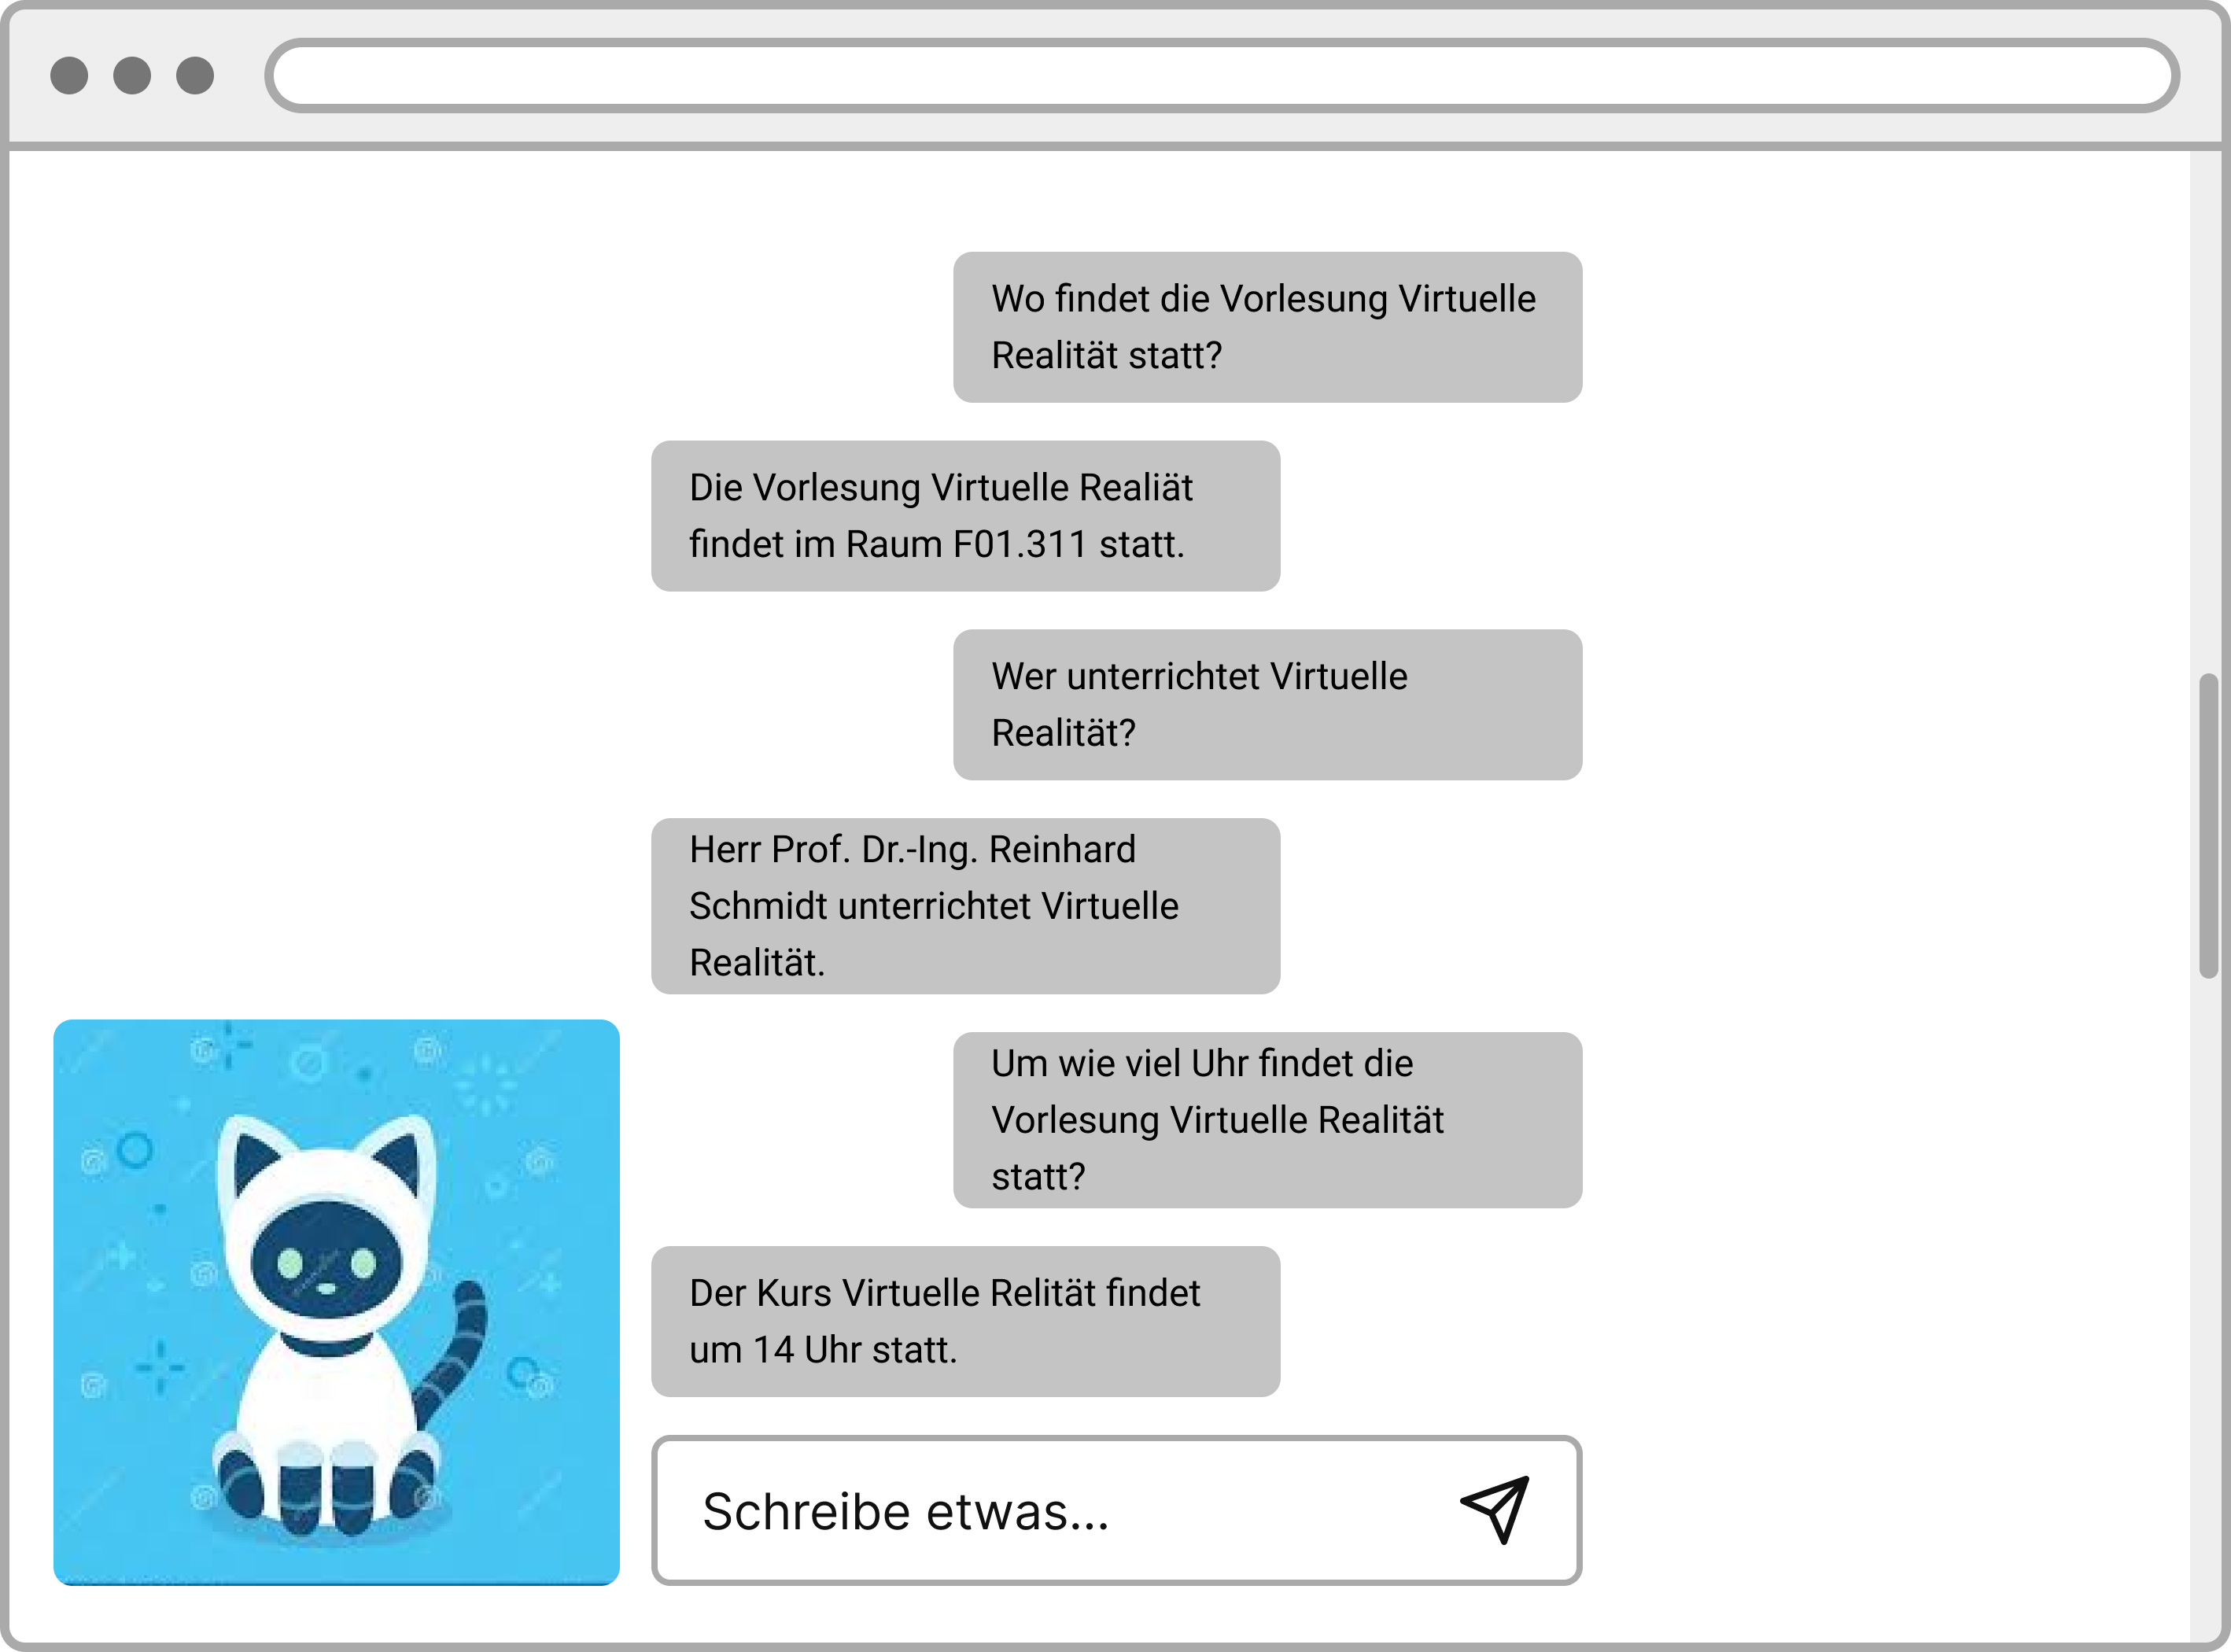
\includegraphics[width=0.8\textwidth]{bilder/new vers. UI Design/WebChat/WebChat Hochschule.png}
    \caption{New version UI Design Webchat Hochschuldomäne}
    \label{fig:New version UI Design Webchat Hochschuldomäne}
    \end{figure}
\noindent \textbf{Webchat mit der Hochschuldomäne} \newline
Diesmal haben wir konkrete Hochschulfragen gestellt und die Hochschuldomäne dargestellt.

\begin{figure}[H]
    \centering
    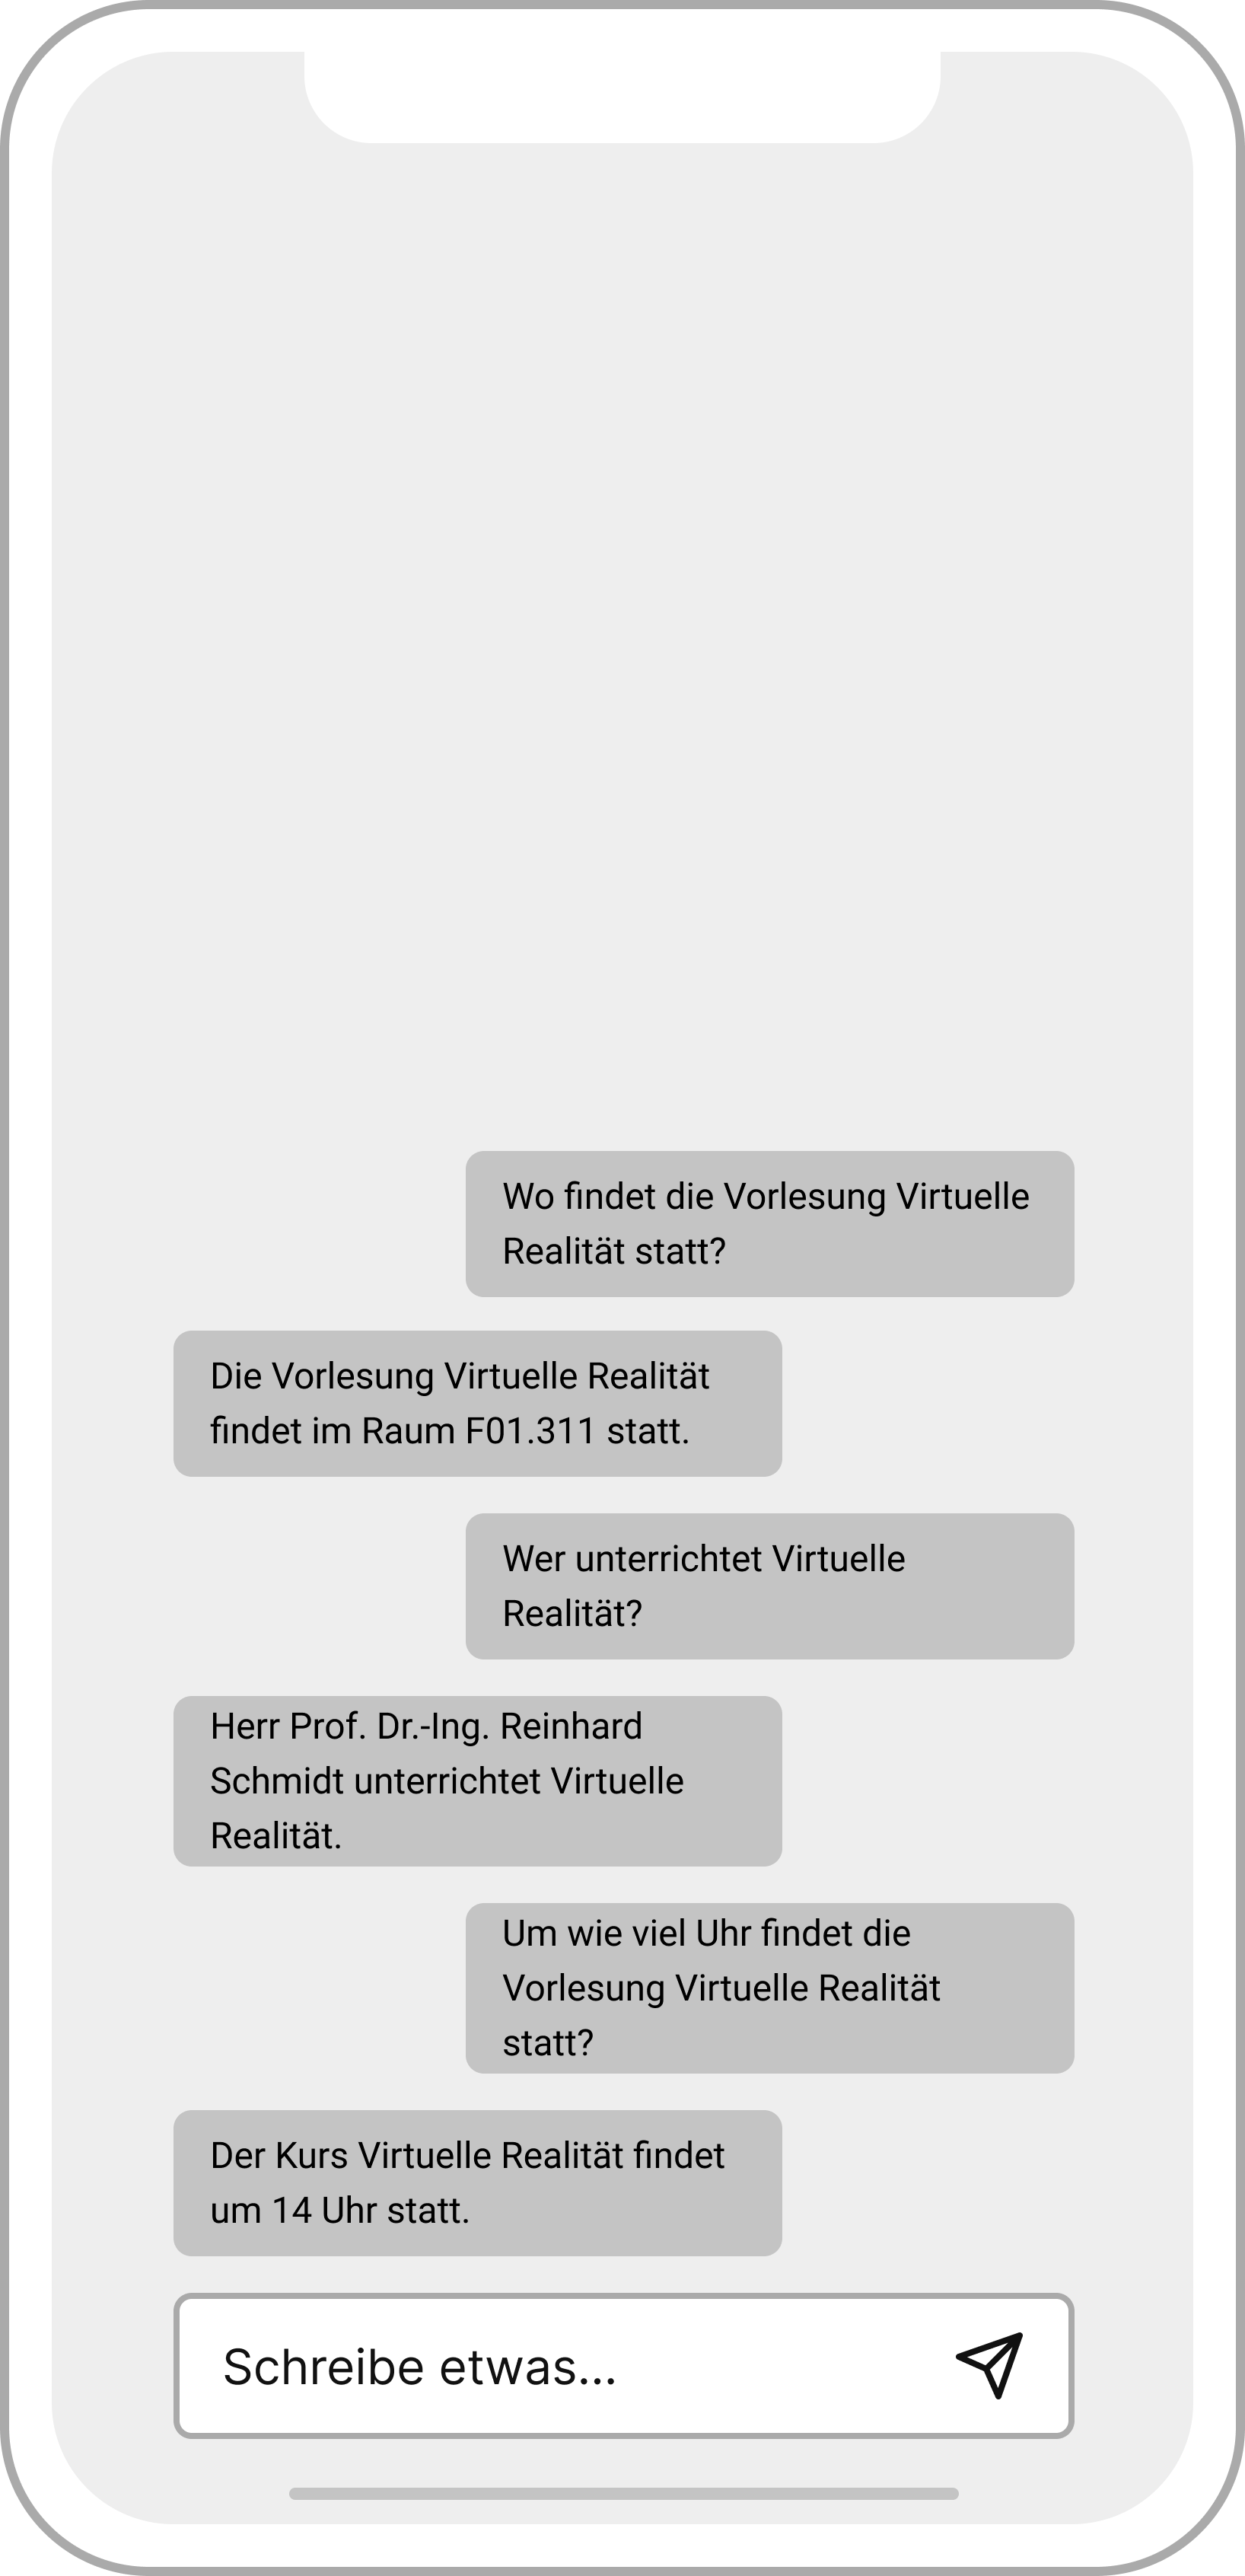
\includegraphics[width=0.5\textwidth]{bilder/new vers. UI Design/WebChat/mobile Version Webchat.png}
    \caption{New version UI Design Webchat mobile version}
    \label{fig:New version UI Design Webchat mobile version}
    \end{figure}
\noindent \textbf{Webchat als mobile Version} \newline
Dies ist die mobile Version des Webchats. Wir haben die Darstellung so einfach wie möglich dargestellt.
Hier haben wir auch die Hochschulbezogenen Fragen gestellt.

\newpage

\subsubsection{Version 2 Admin Interface Allgemein}
Hier werden die neueren Versionen des UI Designs für das Admin-Interface Allgemein vorgestellt

\begin{figure}[H]
    \centering
    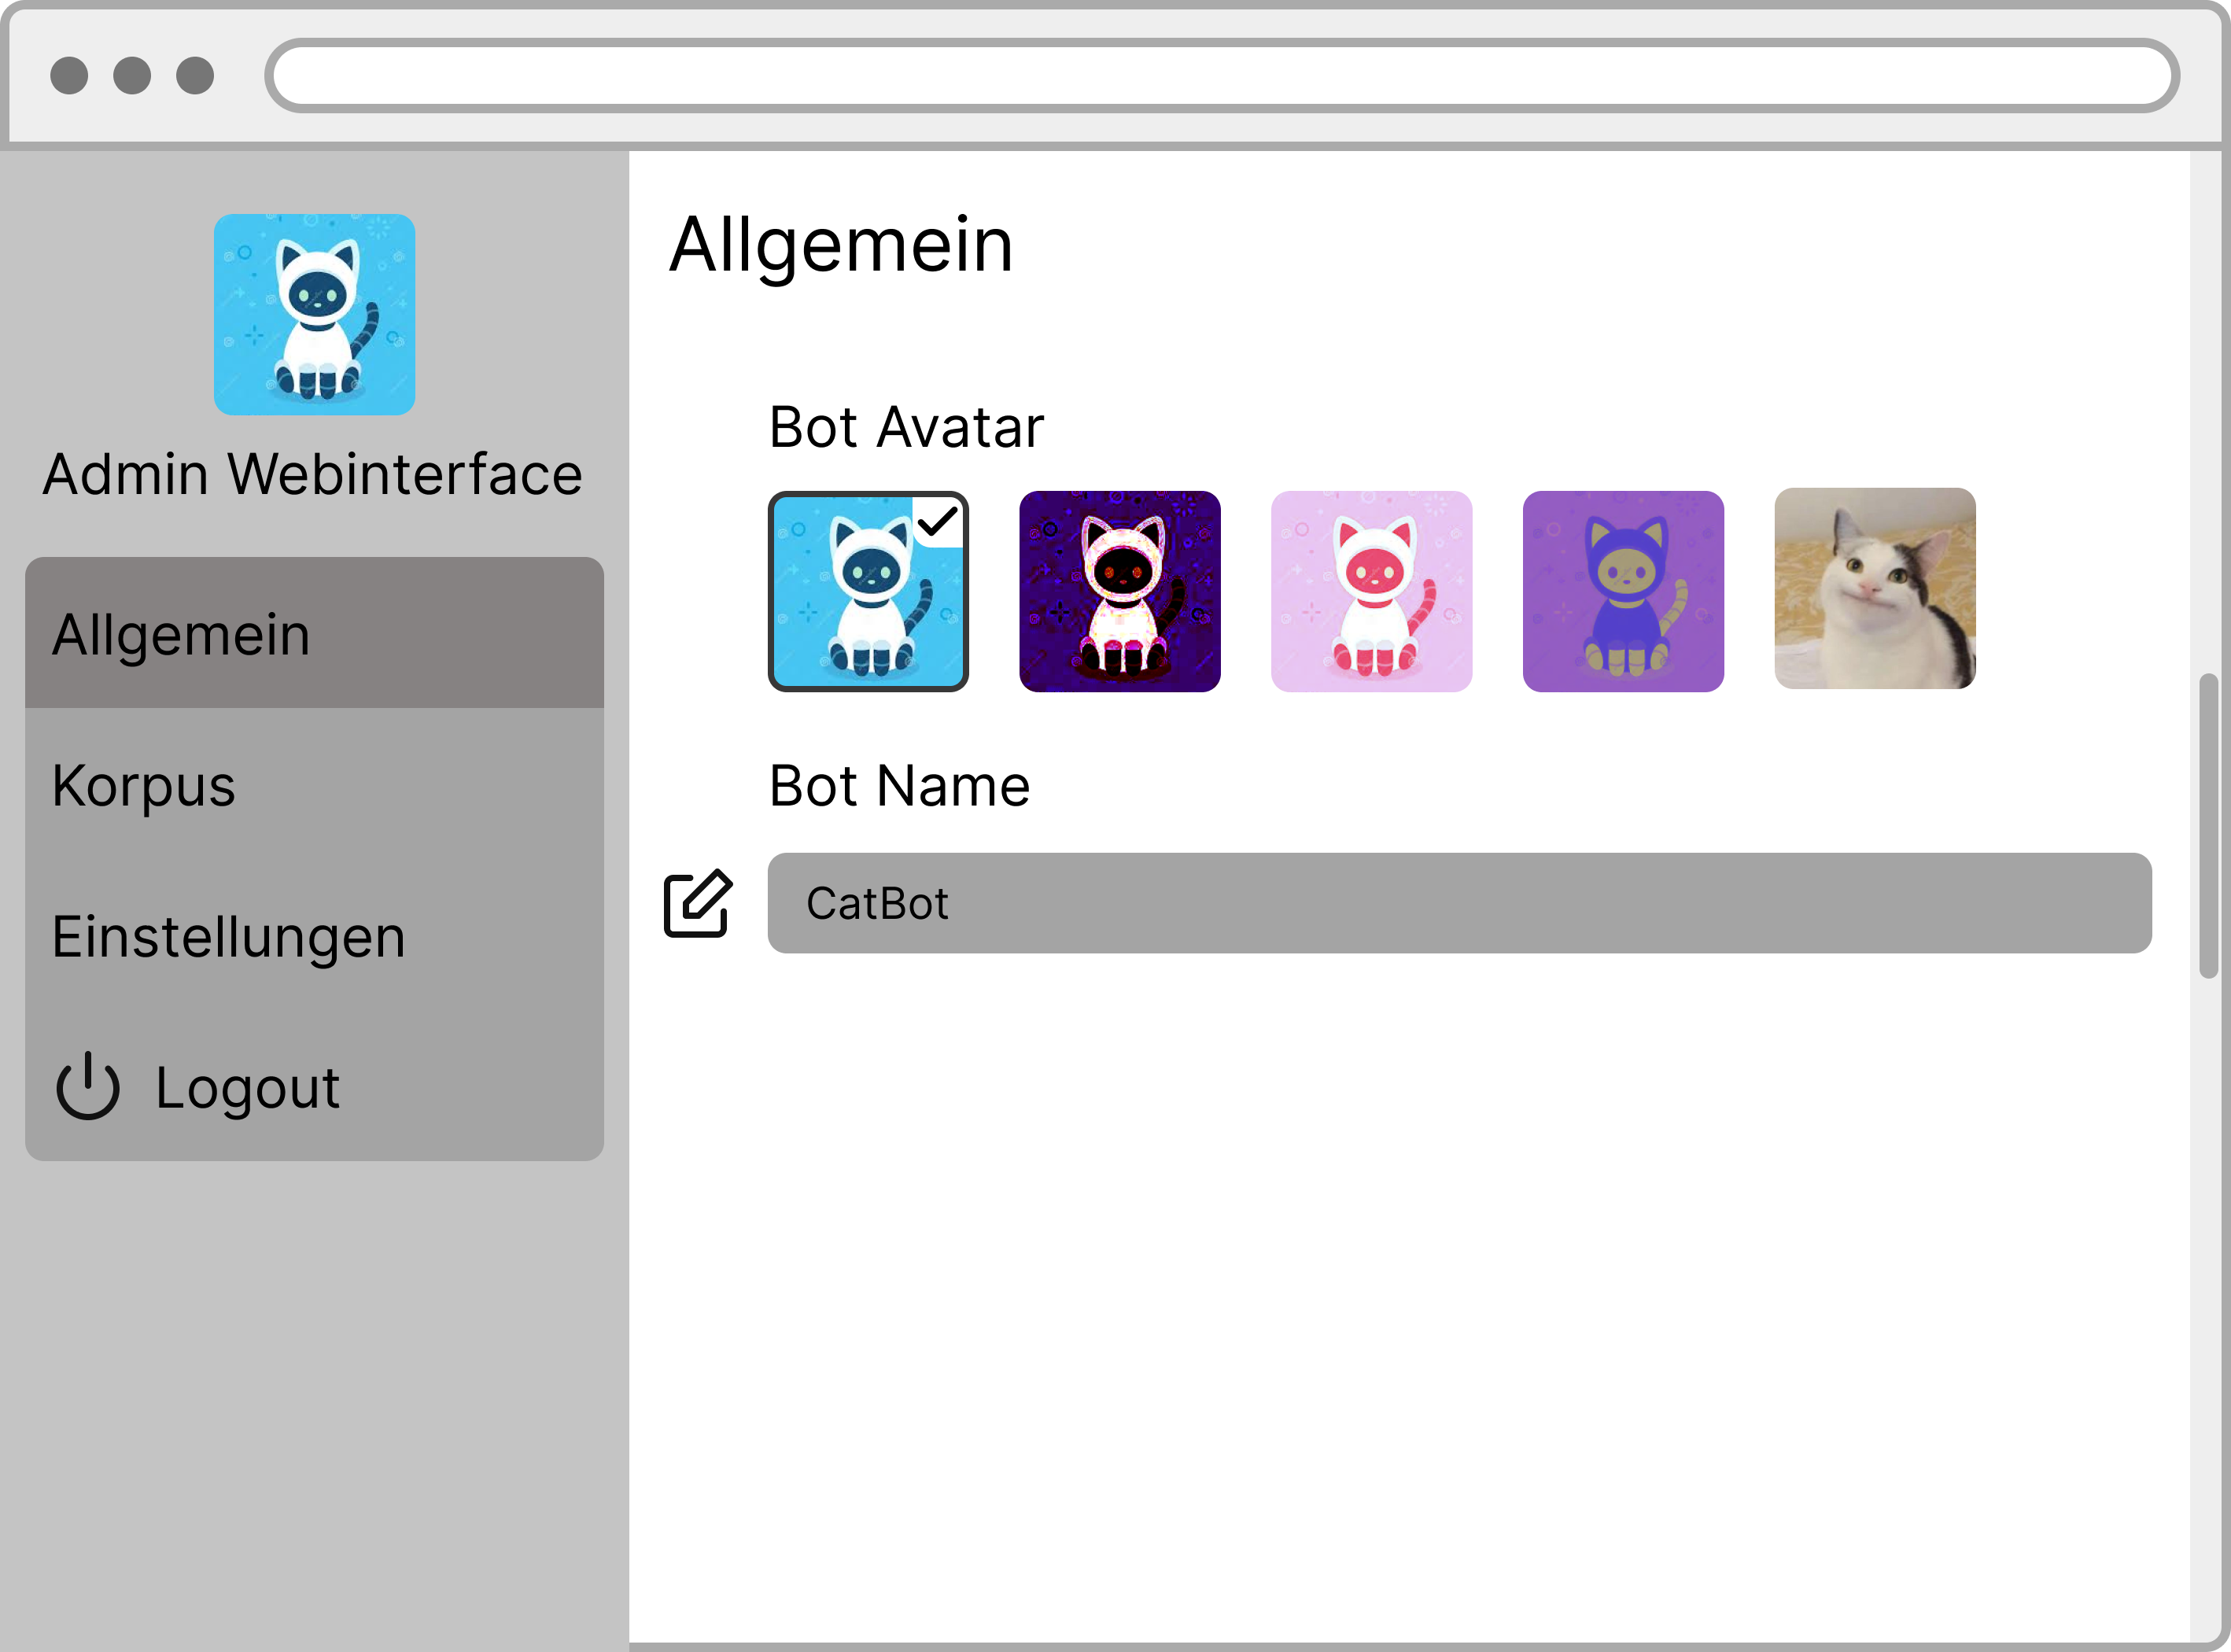
\includegraphics[width=0.8\textwidth]{bilder/new vers. UI Design/Allgemein/Allgemein.png}
    \caption{New version UI Design Admin-Interface Allgemein}
    \label{fig:New version UI Design Admin-Interface Allgemein}
    \end{figure}
\noindent \textbf{Admin Webinterface: Allgemein} \newline
Auf der linken Seite sieht man die Kategorien, die der Admin bearbeiten kann. Im Allgemeinen kann
der Admin den Bot Avatar wechseln, dieser wird dann mit einem Haken gekennzeichnet. Außerdem kann
der Admin den Bot Namen ändern, indem er den Editierbutton drückt.

\begin{figure}[H]
    \centering
    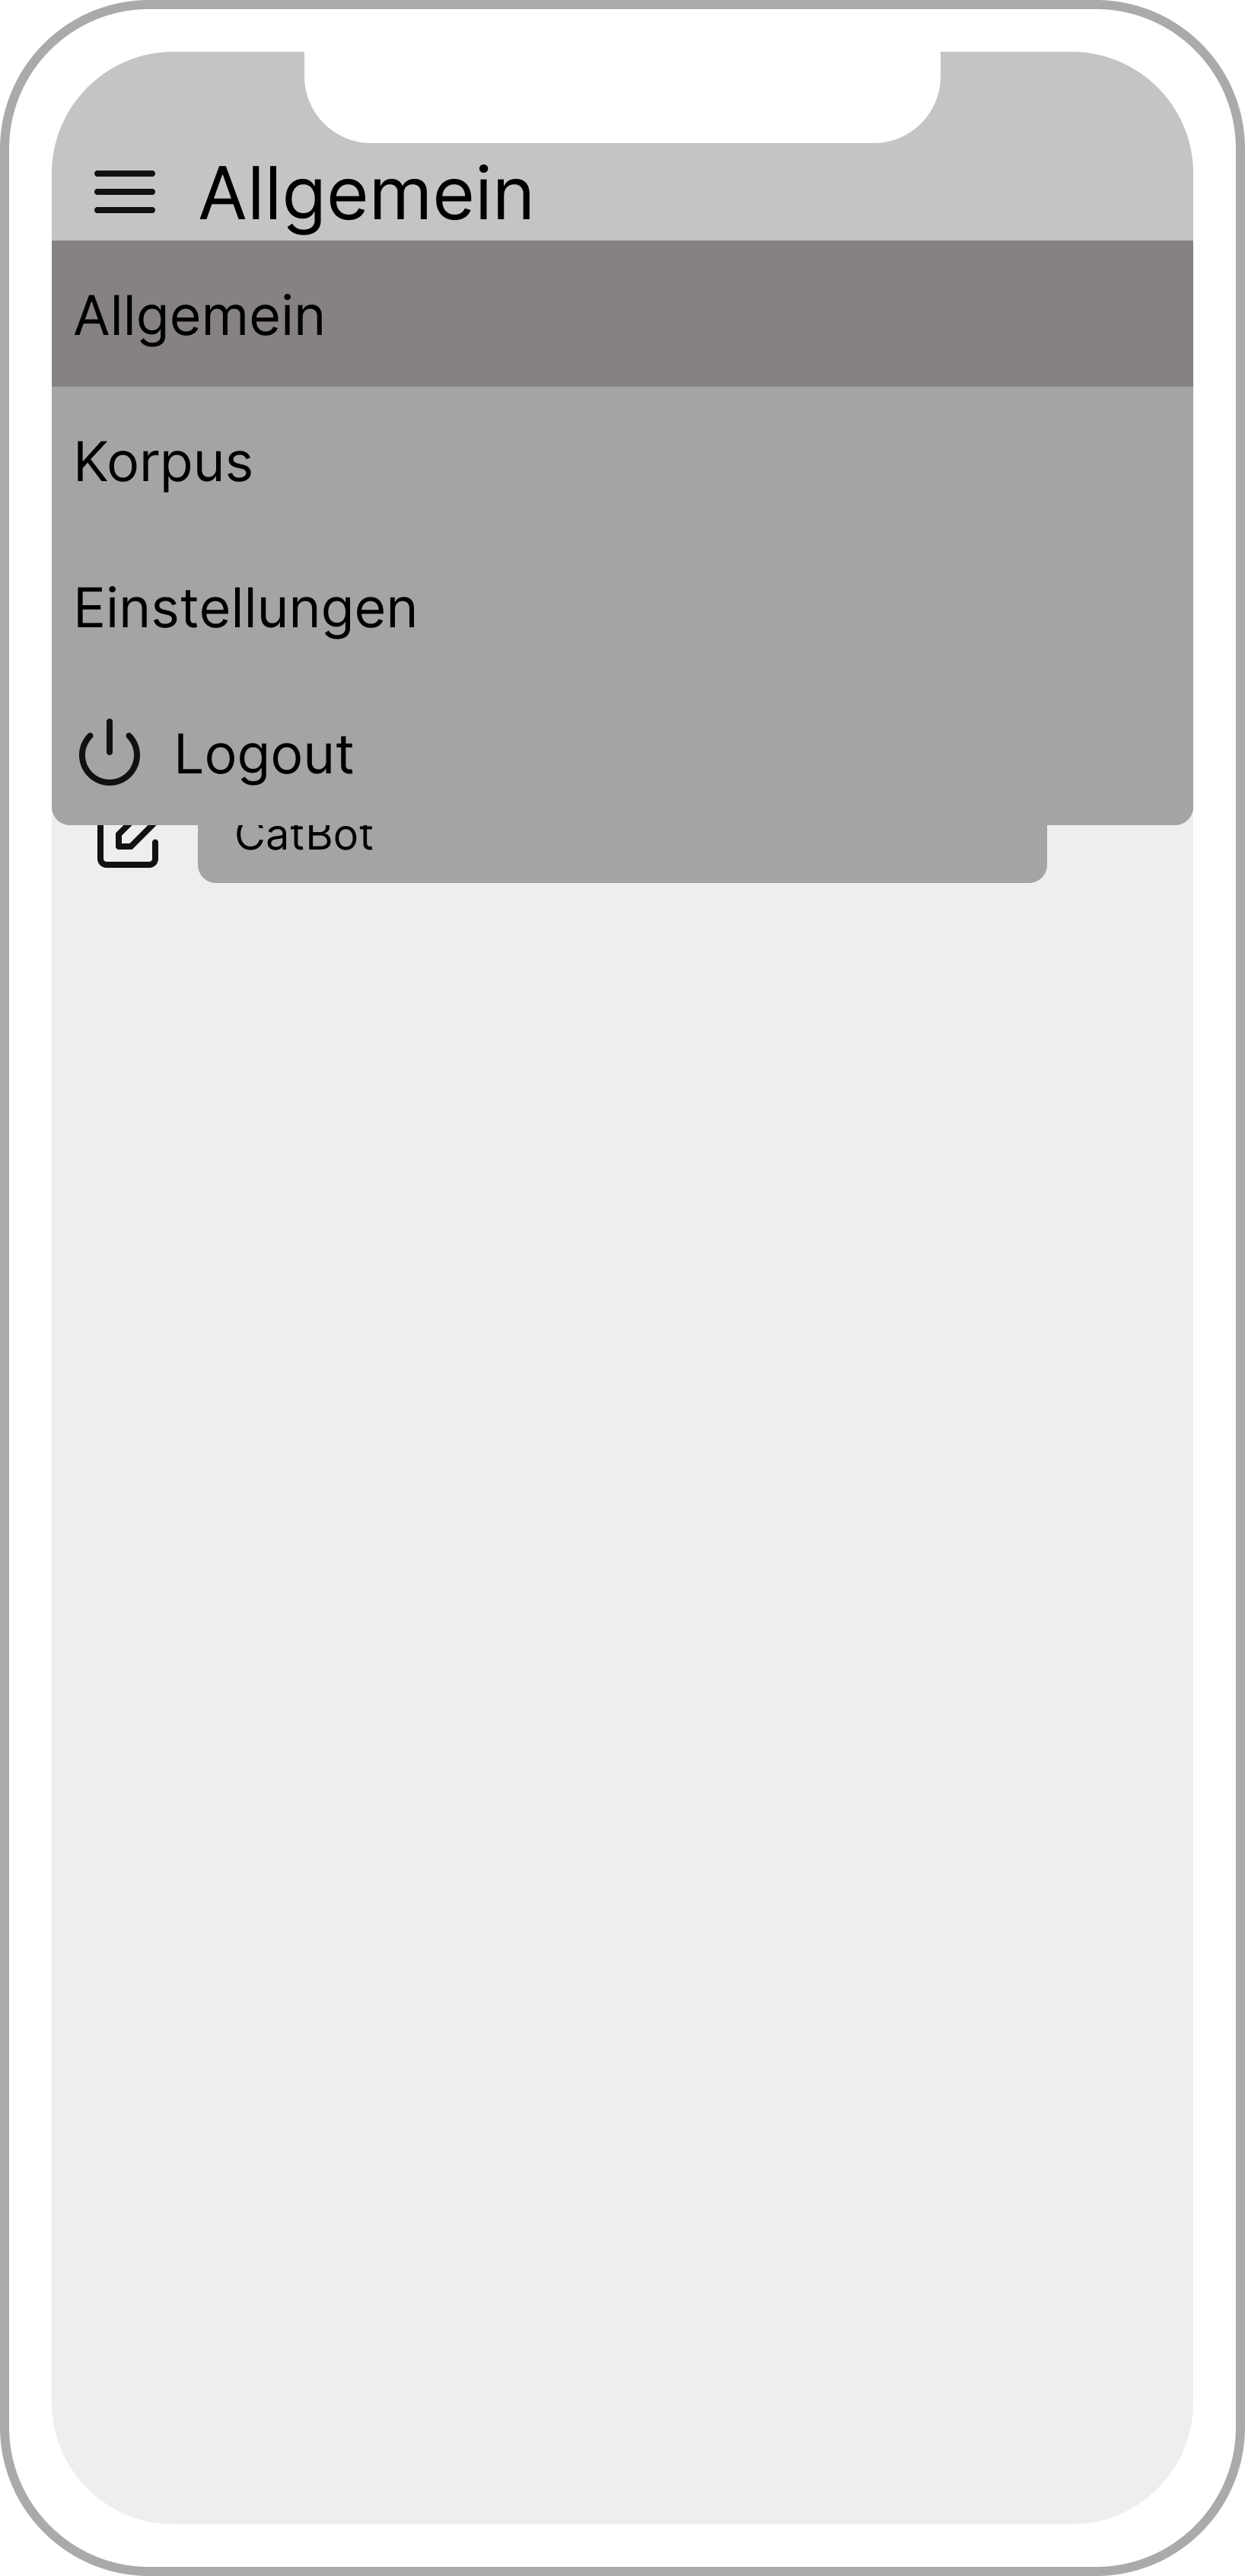
\includegraphics[width=0.5\textwidth]{bilder/new vers. UI Design/Allgemein/iPhone X Allgemein dropdown.png}
    \caption{New version UI Design Admin-Interface Allgemein dropdown menu}
    \label{fig:New version UI Design Admin-Interface Allgemein dropdown menu}
\end{figure}
\noindent \textbf{Admin Webinterface mobil: Allgemein dropdown Menü} \newline
In der mobilen Version haben wir die Kategorien, die der Admin bearbeiten kann im dropdown Menü dargestellt.

\begin{figure}[H]
    \centering
    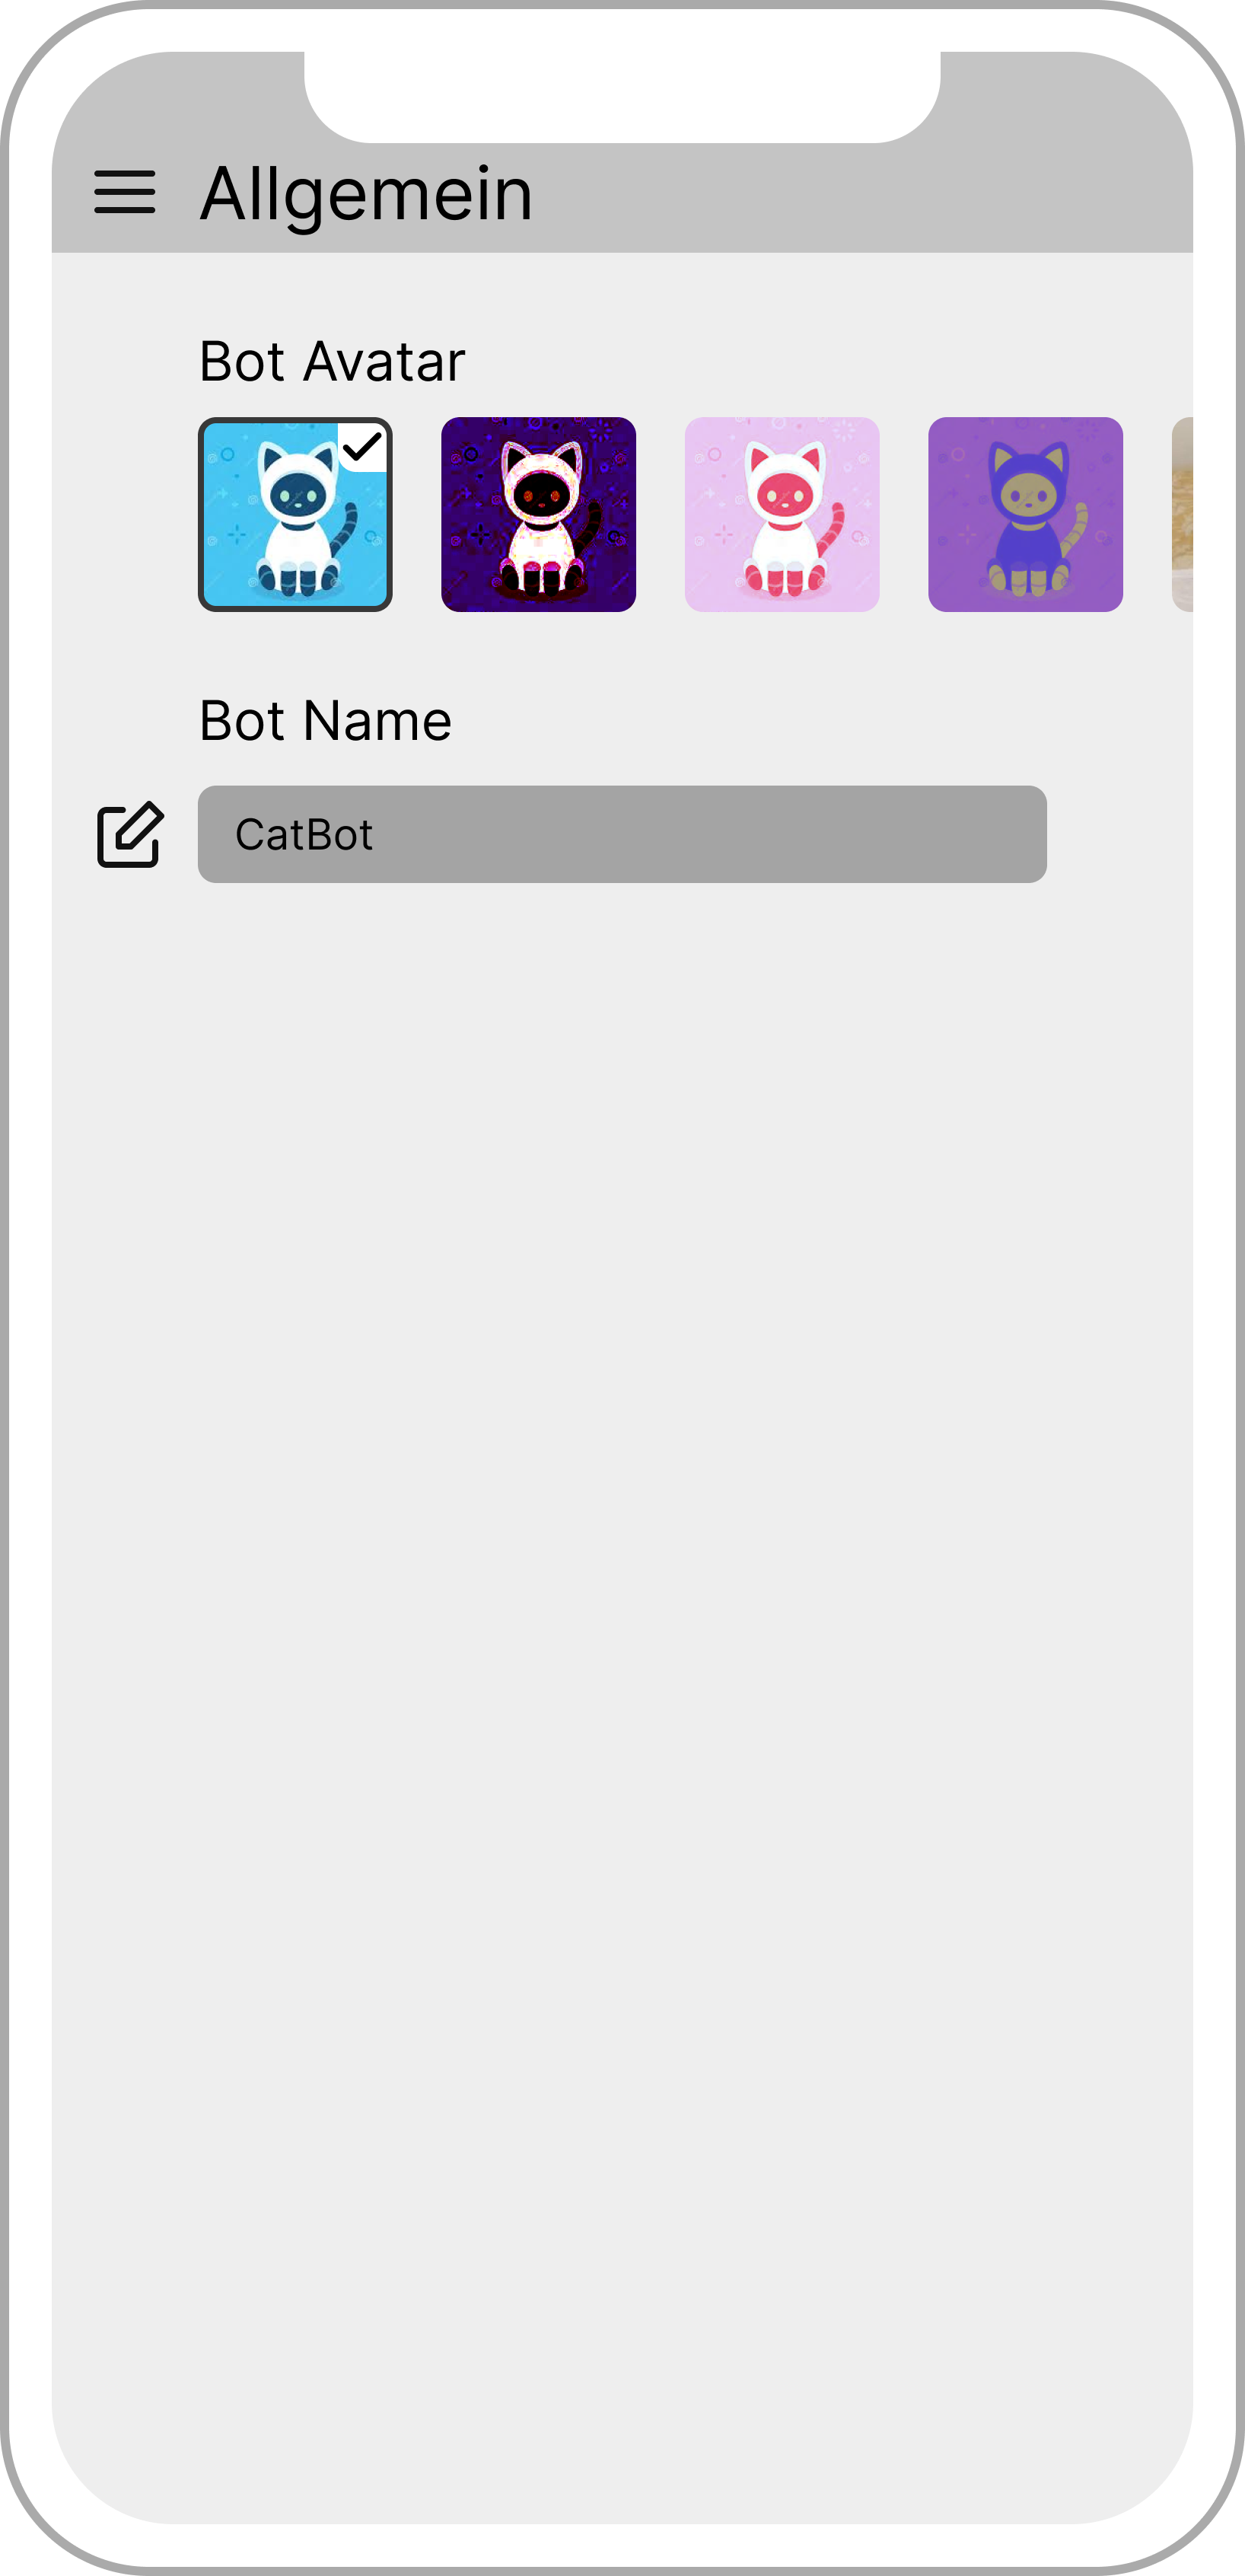
\includegraphics[width=0.5\textwidth]{bilder/new vers. UI Design/Allgemein/iPhone X Allgemein III.png}
    \caption{New version UI Design Admin-Interface Allgemein mobile version}
    \label{fig:New version UI Design Admin-Interface Allgemein mobile version}
\end{figure}
\noindent \textbf{Admin Webinterface mobil: Allgemein} \newline
Die mobile Variante funktioniert genauso wie die Webvariante. Man kann den Bot Avatar wechseln und den
ChatBot Namen frei bestimmen.

\newpage

\subsubsection{Version 2 Admin Interface Korpus}
Hier werden die neueren Versionen des UI Designs für das Admin-Interface Korpus vorgestellt.

\begin{figure}[H]
    \centering
    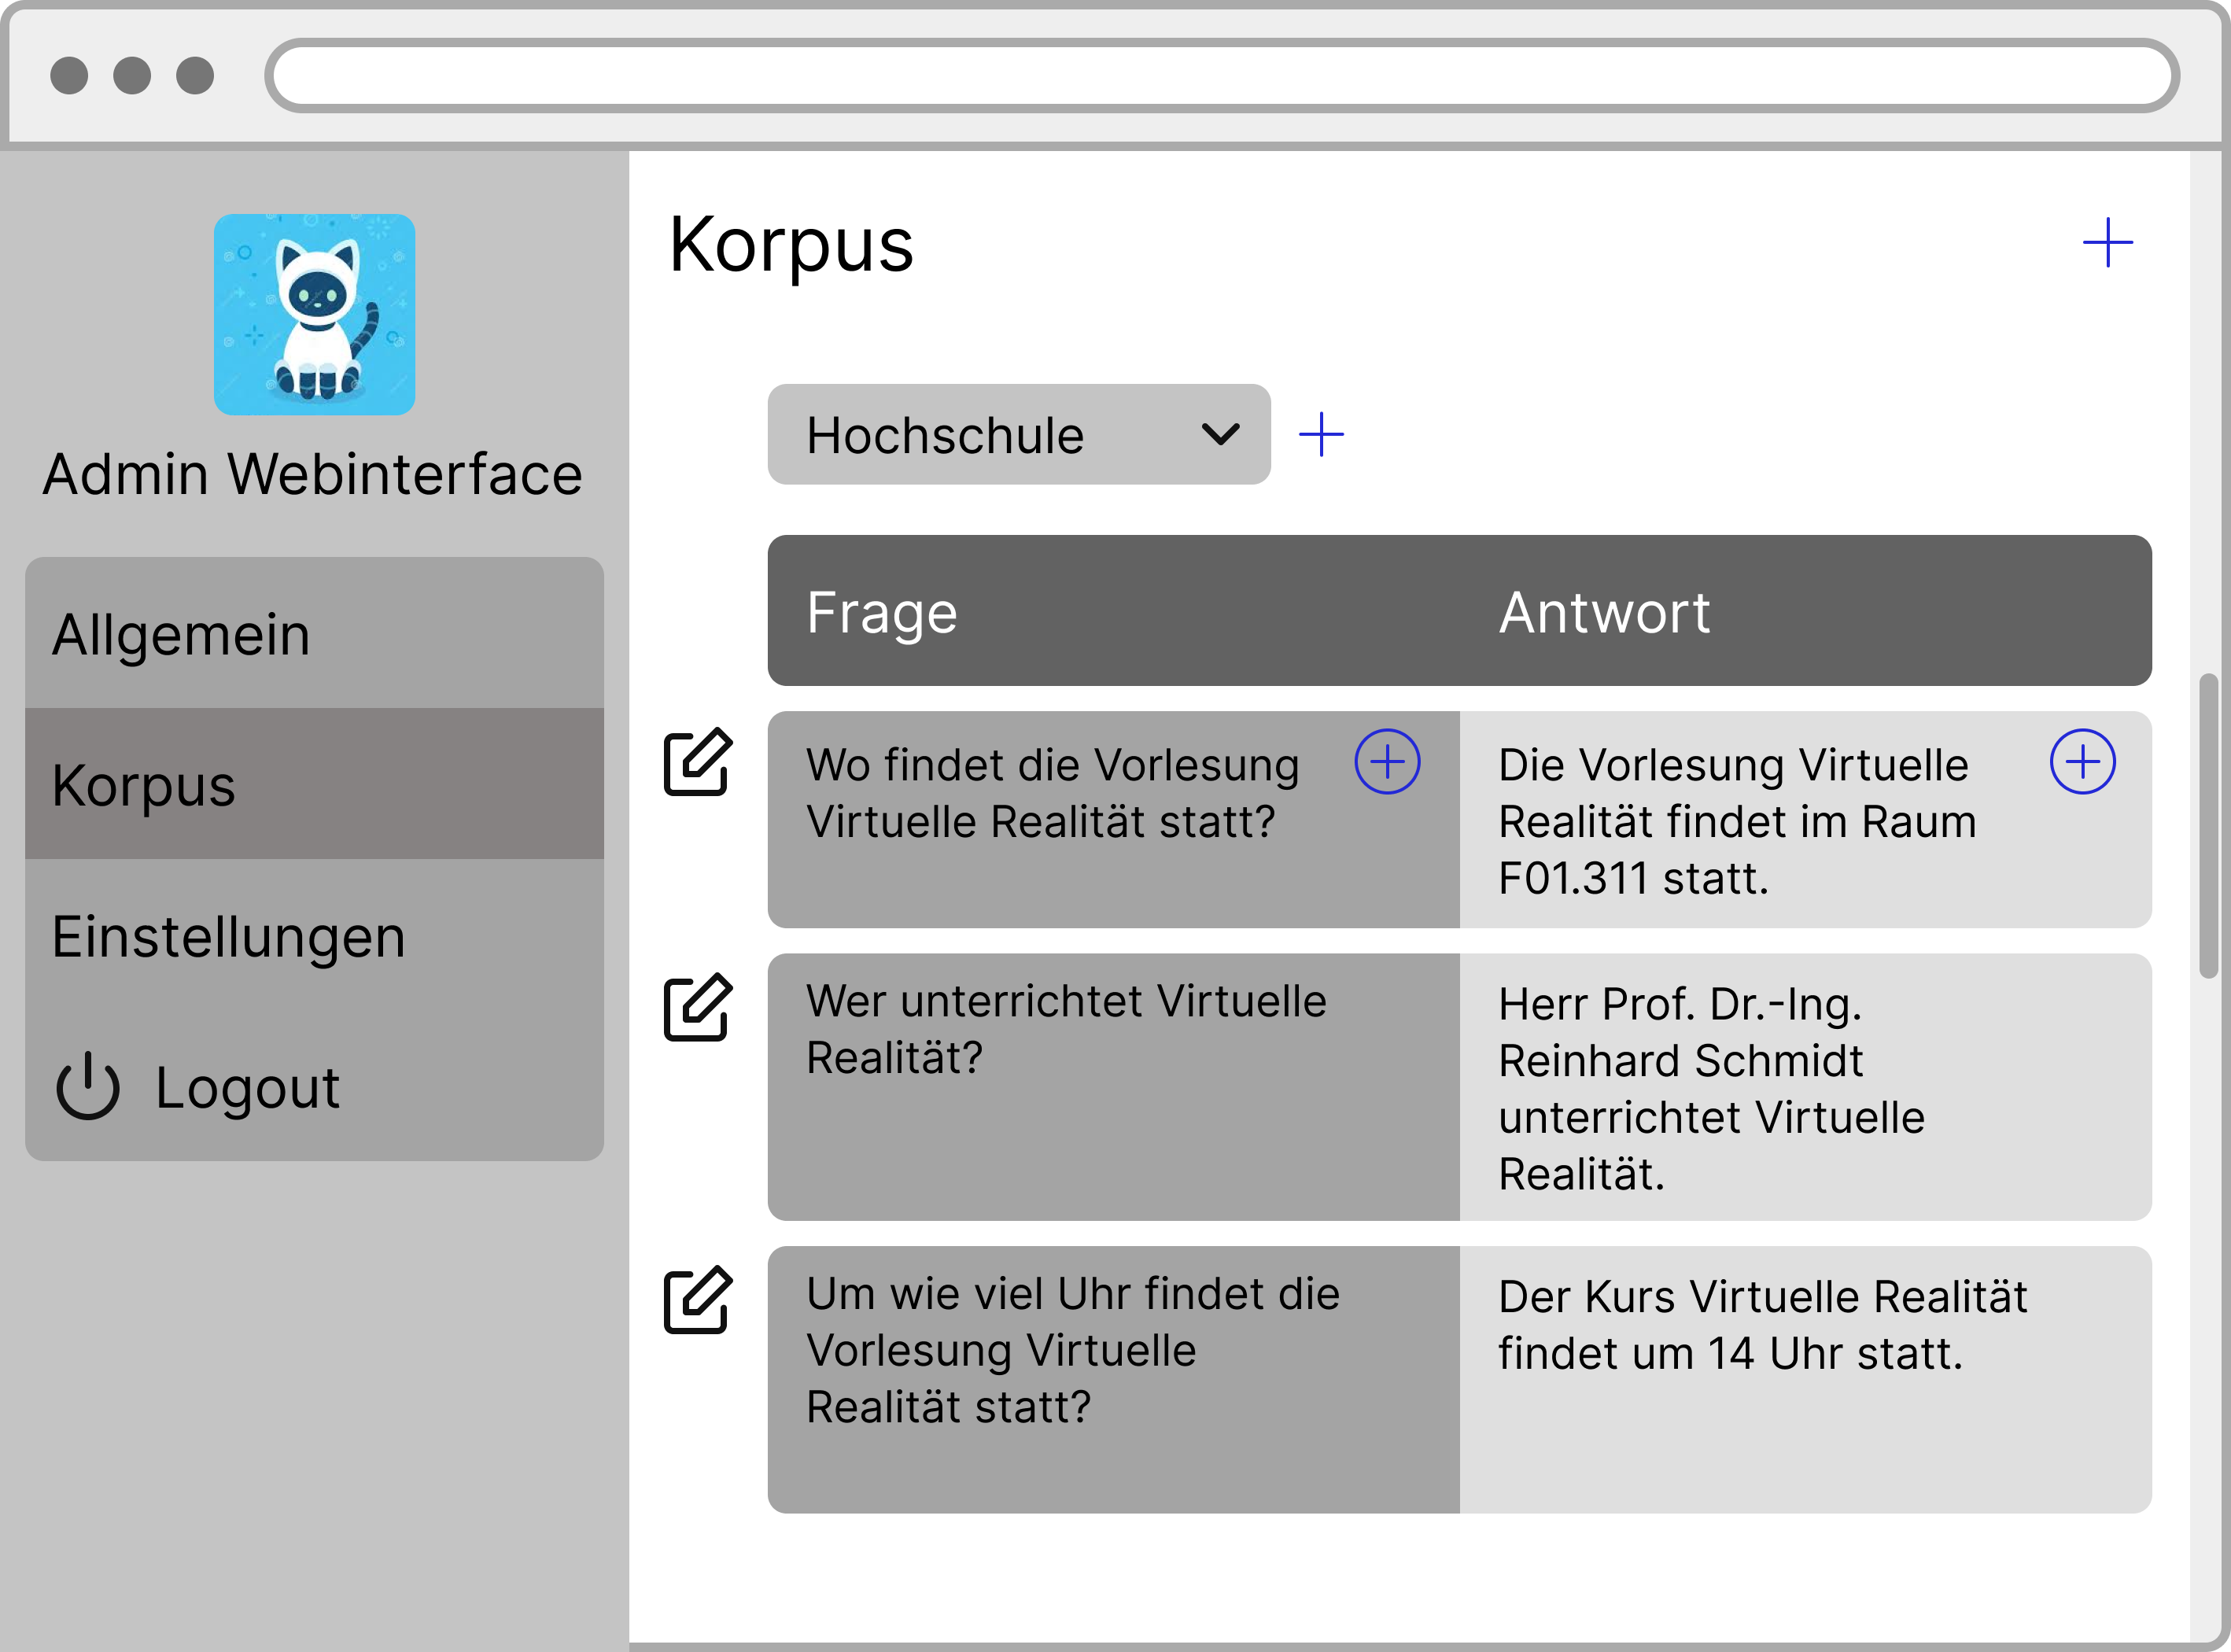
\includegraphics[width=1.0\textwidth]{bilder/new vers. UI Design/Korpus/Admin Interface 00.png}
    \caption{New version UI Design Admin-Interface Korpus 00}
    \label{fig:New version UI Design Admin-Interface Korpus 00}
\end{figure}
\noindent  \textbf{Admin Webinterface: Korpus 00} \newline
Im Korpus kann der Admin weitere Domänen, Fragen und Antworten einsehen.

\begin{figure}[H]
    \centering
    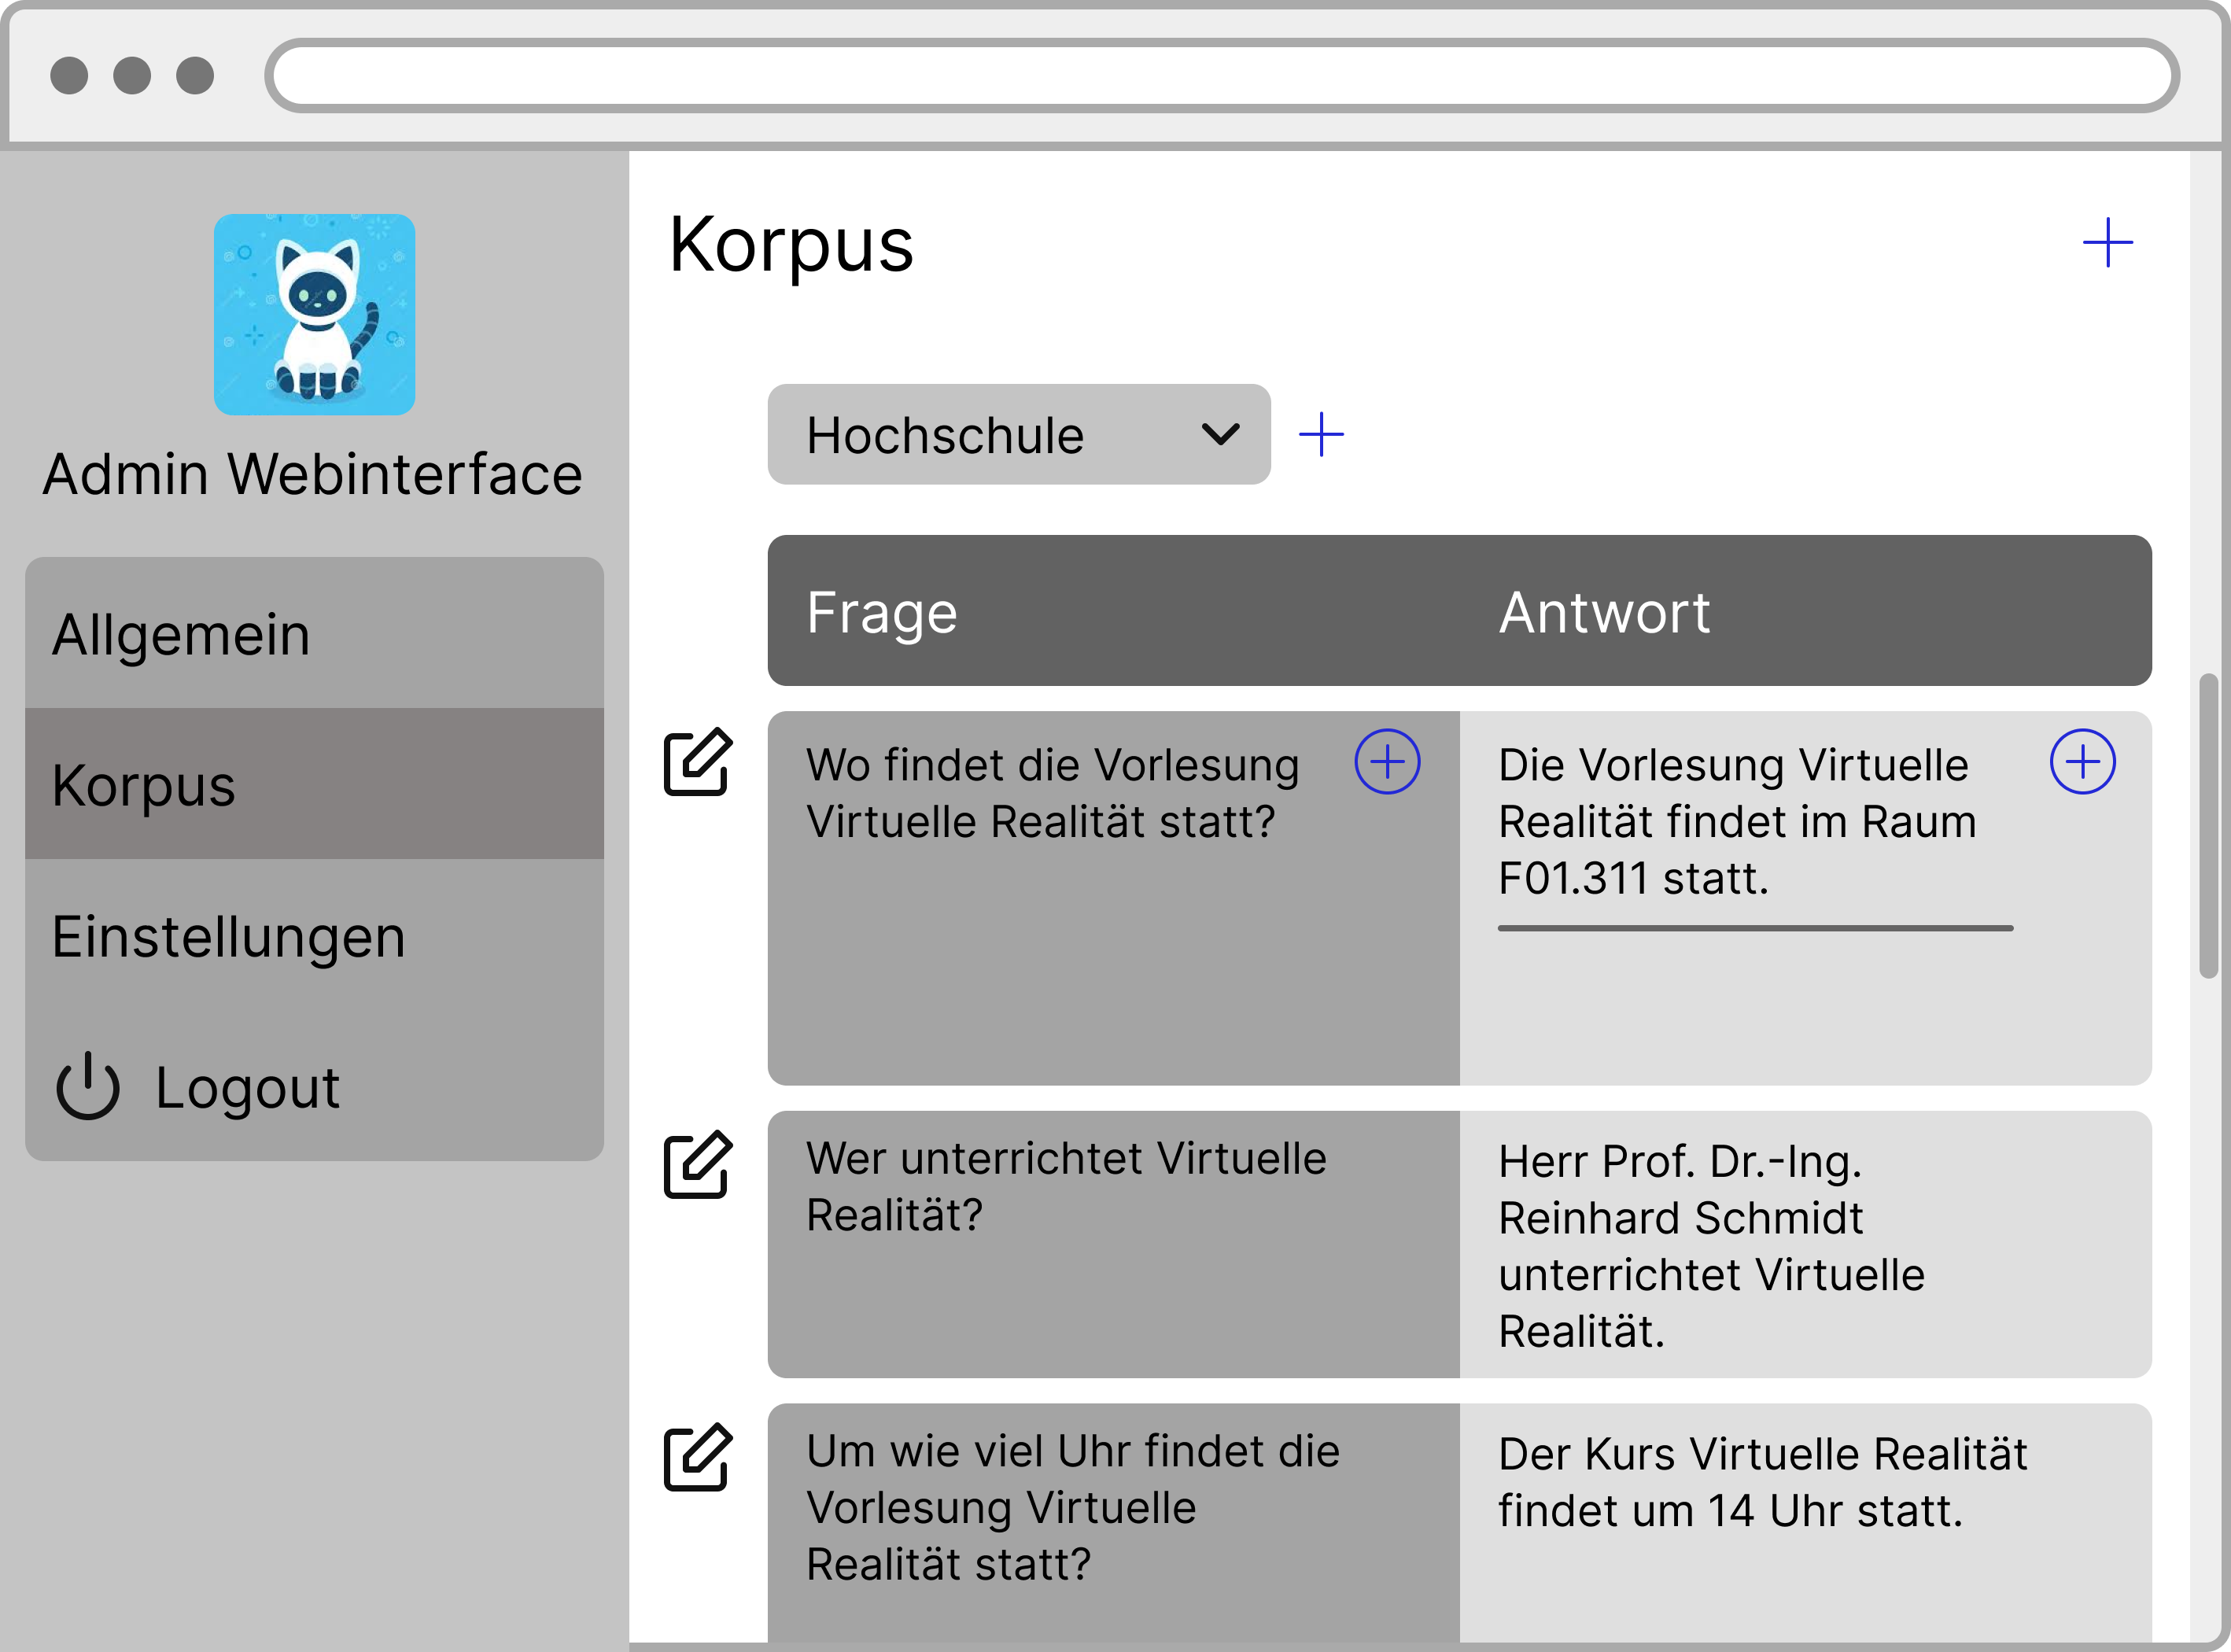
\includegraphics[width=1.0\textwidth]{bilder/new vers. UI Design/Korpus/Admin Interface 01.png}
    \caption{New version UI Design Admin-Interface Korpus 01}
    \label{fig:New version UI Design Admin-Interface Korpus 01}
\end{figure}
\noindent \textbf{Admin Webinterface: Korpus 01} \newline
Mit dem Editierbutton kann er Domänen, Fragen und Antworten hinzufügen und entfernen.

\begin{figure}[H]
    \centering
    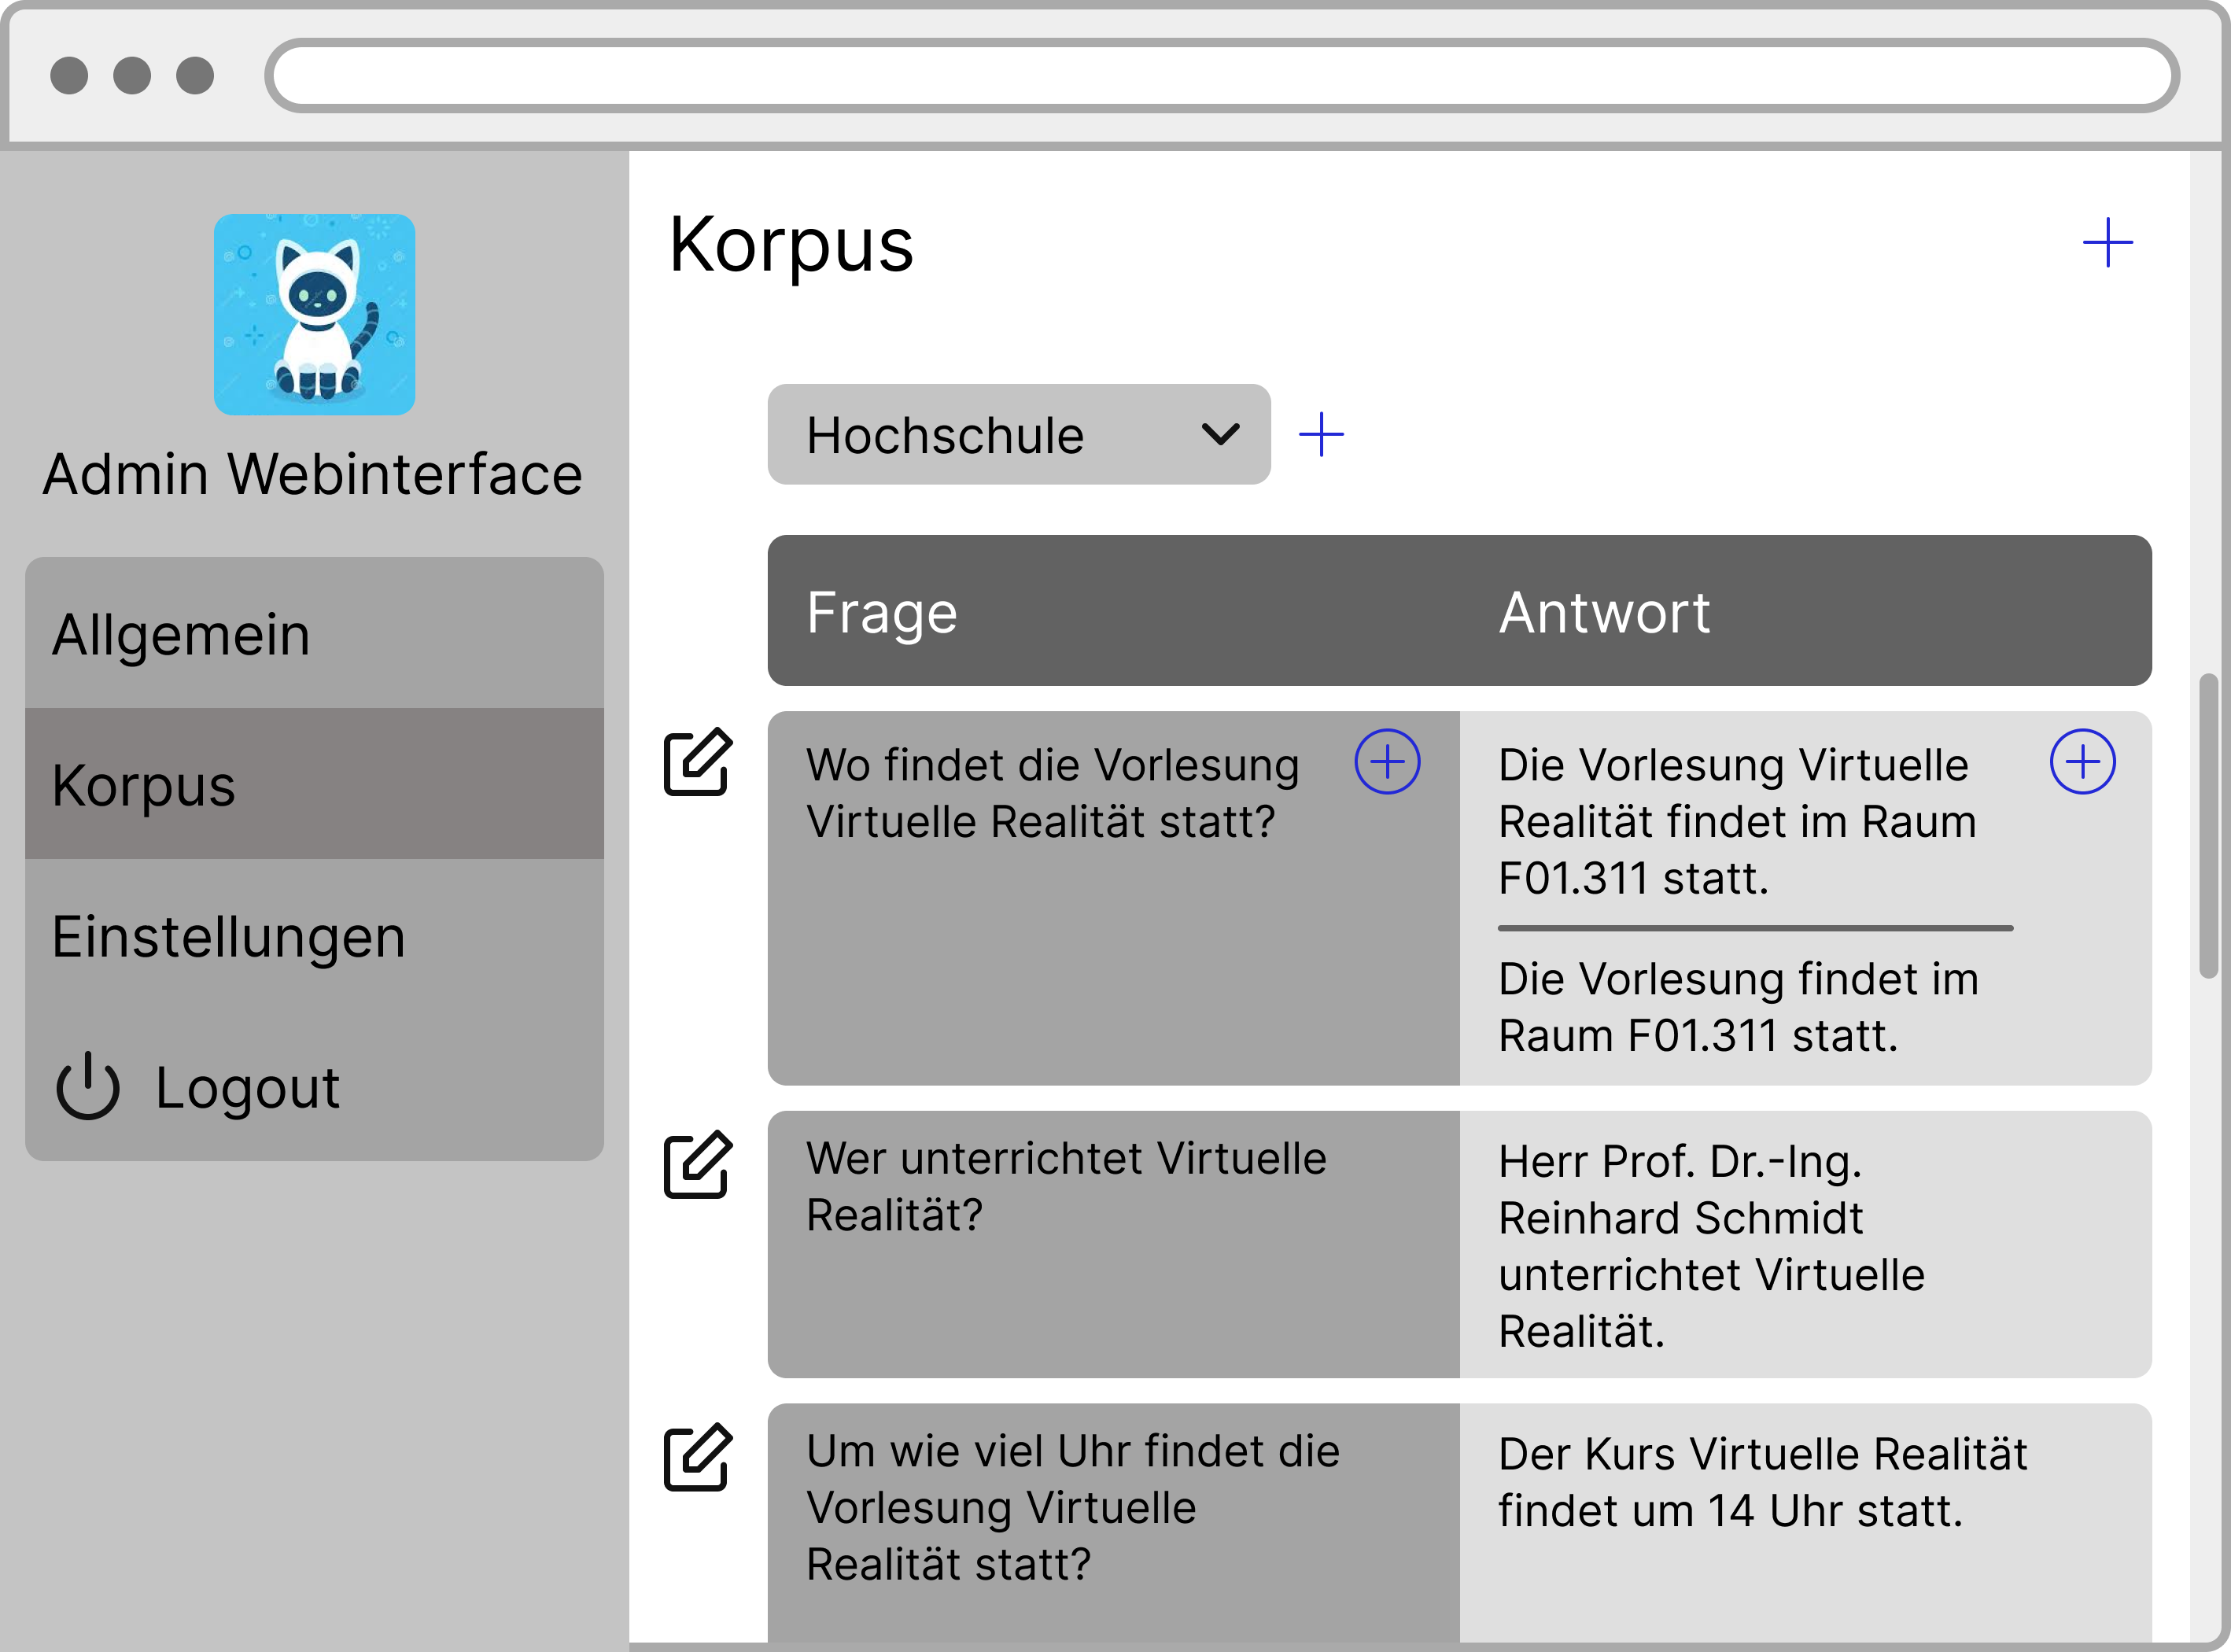
\includegraphics[width=1.0\textwidth]{bilder/new vers. UI Design/Korpus/Admin Interface 02.png}
    \caption{New version UI Design Admin-Interface Korpus 02}
    \label{fig:New version UI Design Admin-Interface Korpus 02}
\end{figure}
\noindent \textbf{Admin Webinterface: Korpus 02} \newline
So kann man wie im Beispiel eine weitere Antwort zu der Frage: "Wo findet die Vorlesung Virtuelle
Realität statt?", hinzufügen.

\begin{figure}[H]
    \centering
    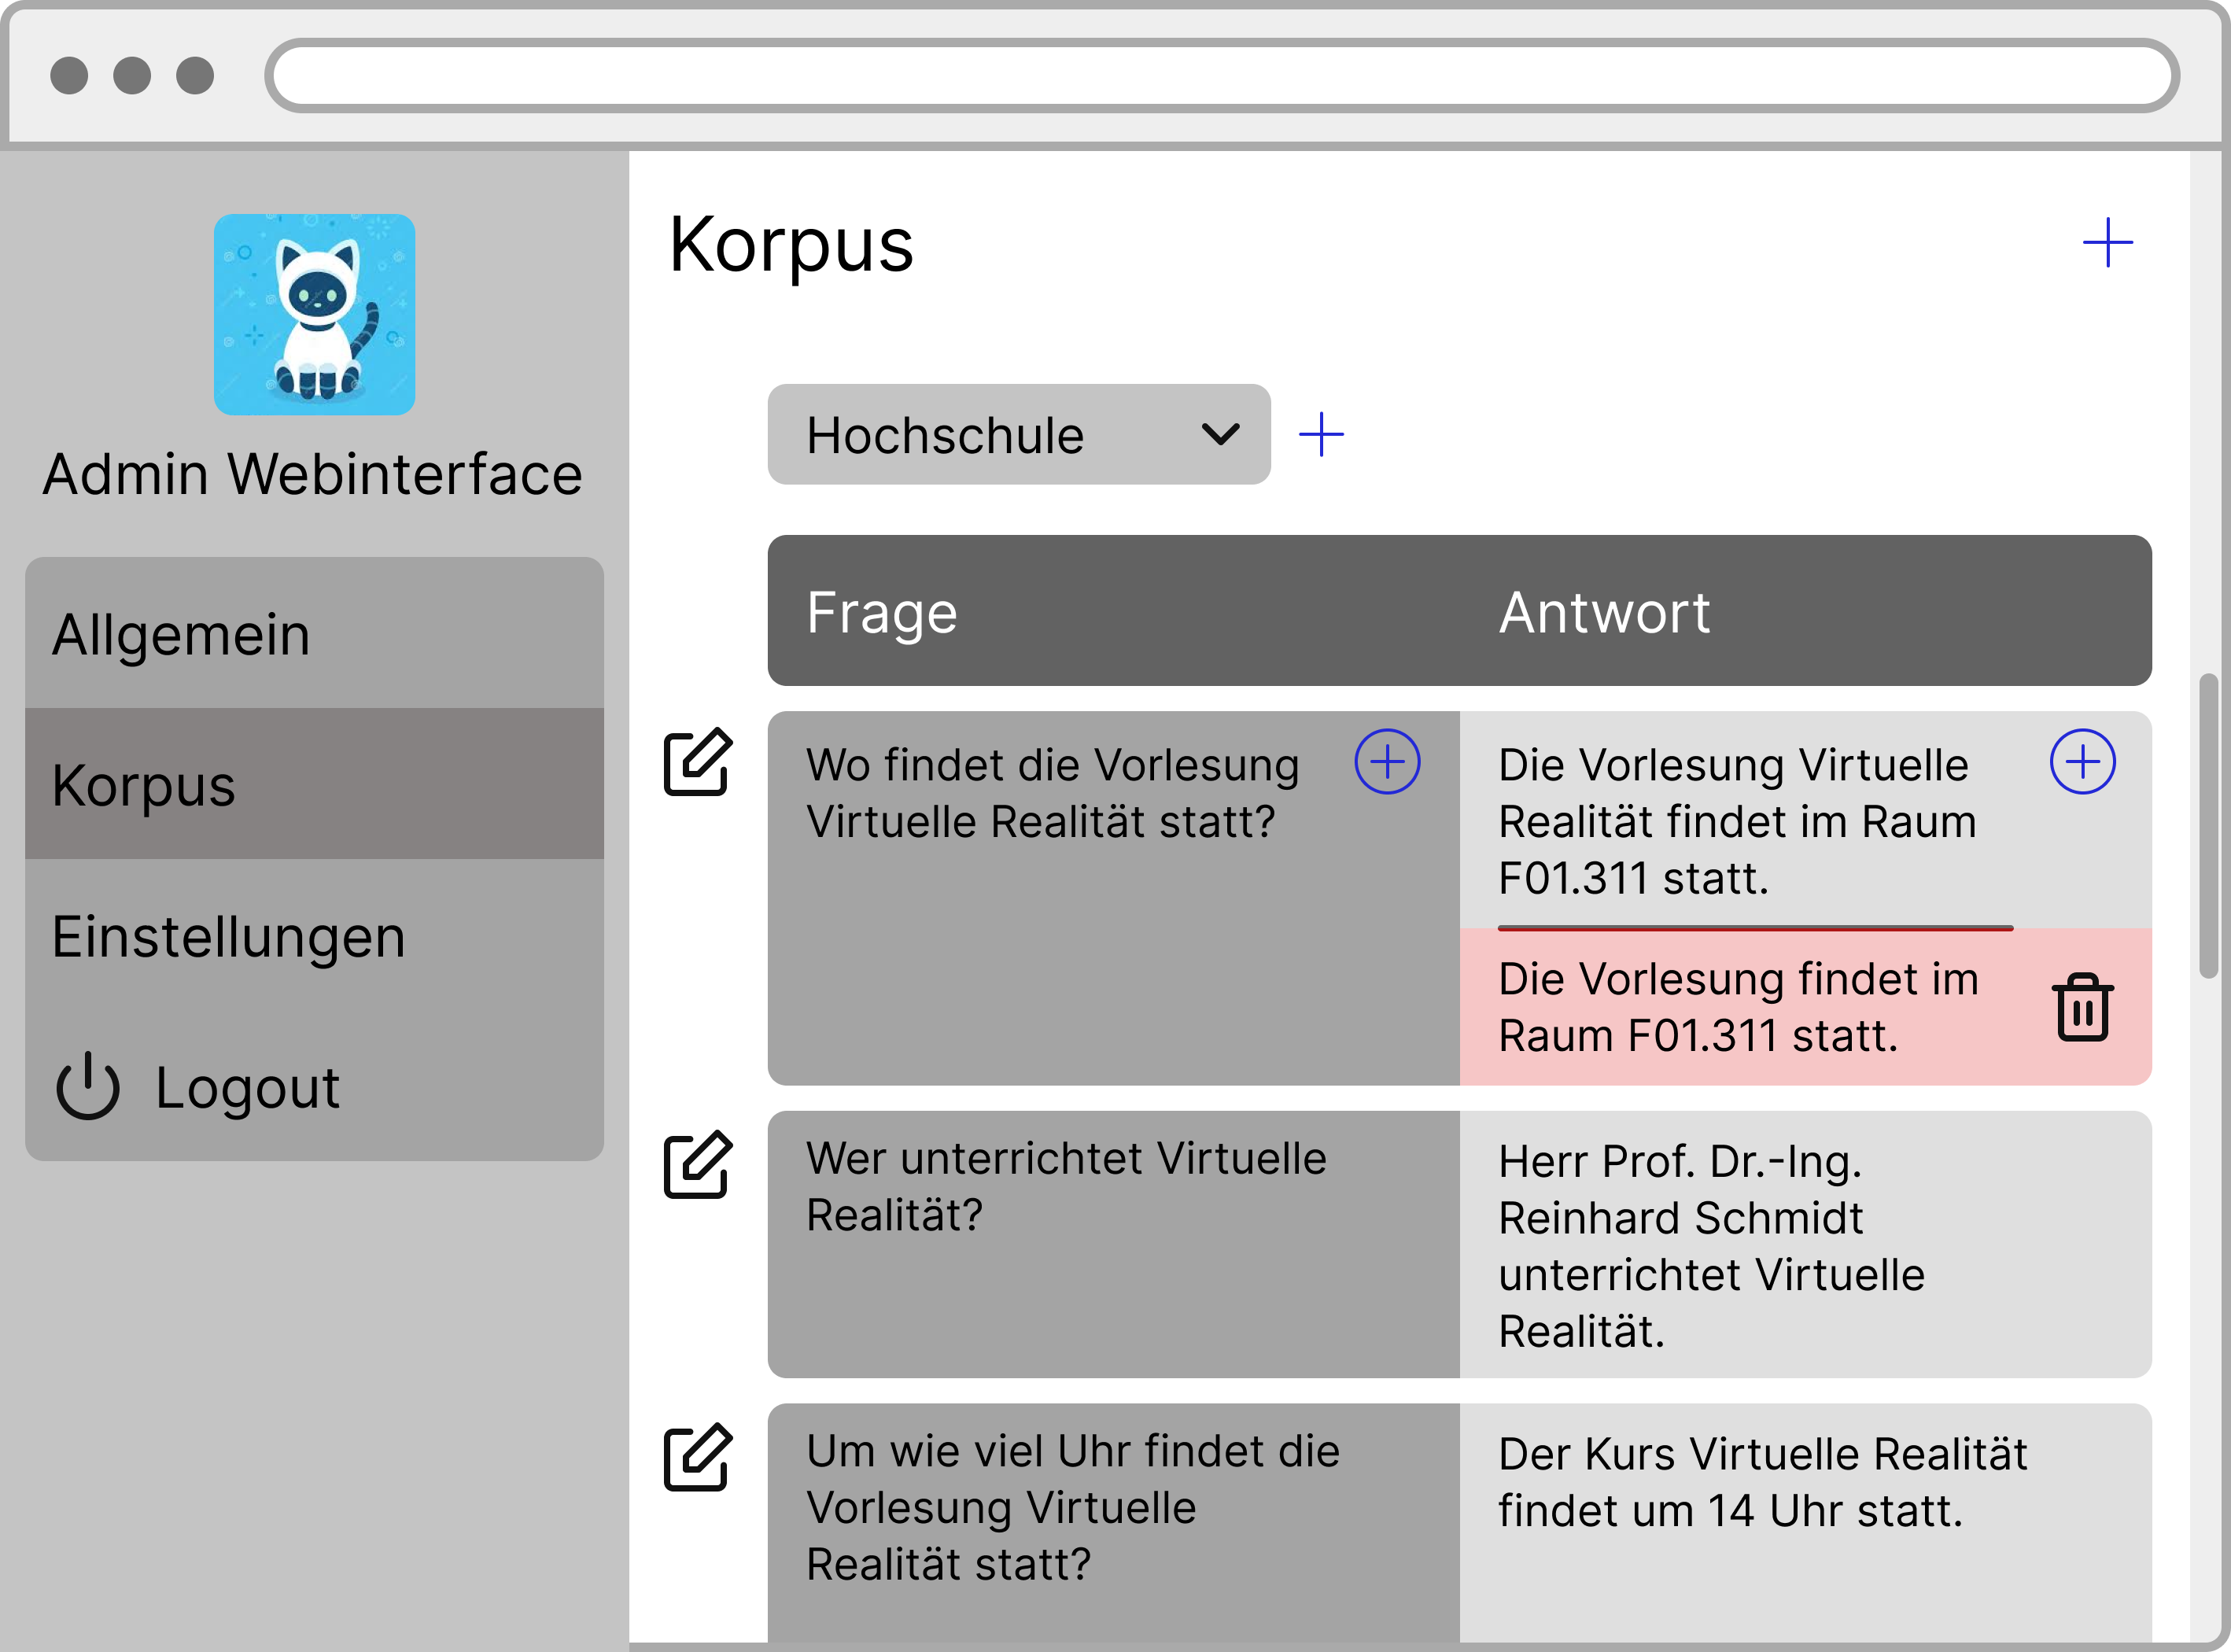
\includegraphics[width=1.0\textwidth]{bilder/new vers. UI Design/Korpus/Admin Interface 03.png}
    \caption{New version UI Design Admin-Interface Korpus 03}
    \label{fig:New version UI Design Admin-Interface Korpus 03}
\end{figure}
\noindent \textbf{Admin Webinterface: Korpus 03} \newline
Natürlich kann man auch die hinzugefügte Antwort entfernen. Man klickt auf das Feld und das Feld erscheint rötlich und ein
Mülleimersymbol entsteht. Wenn man jetzt auf das Eimer-Symbol klickt, kann man die
Antwort löschen.

\begin{figure}[H]
    \centering
    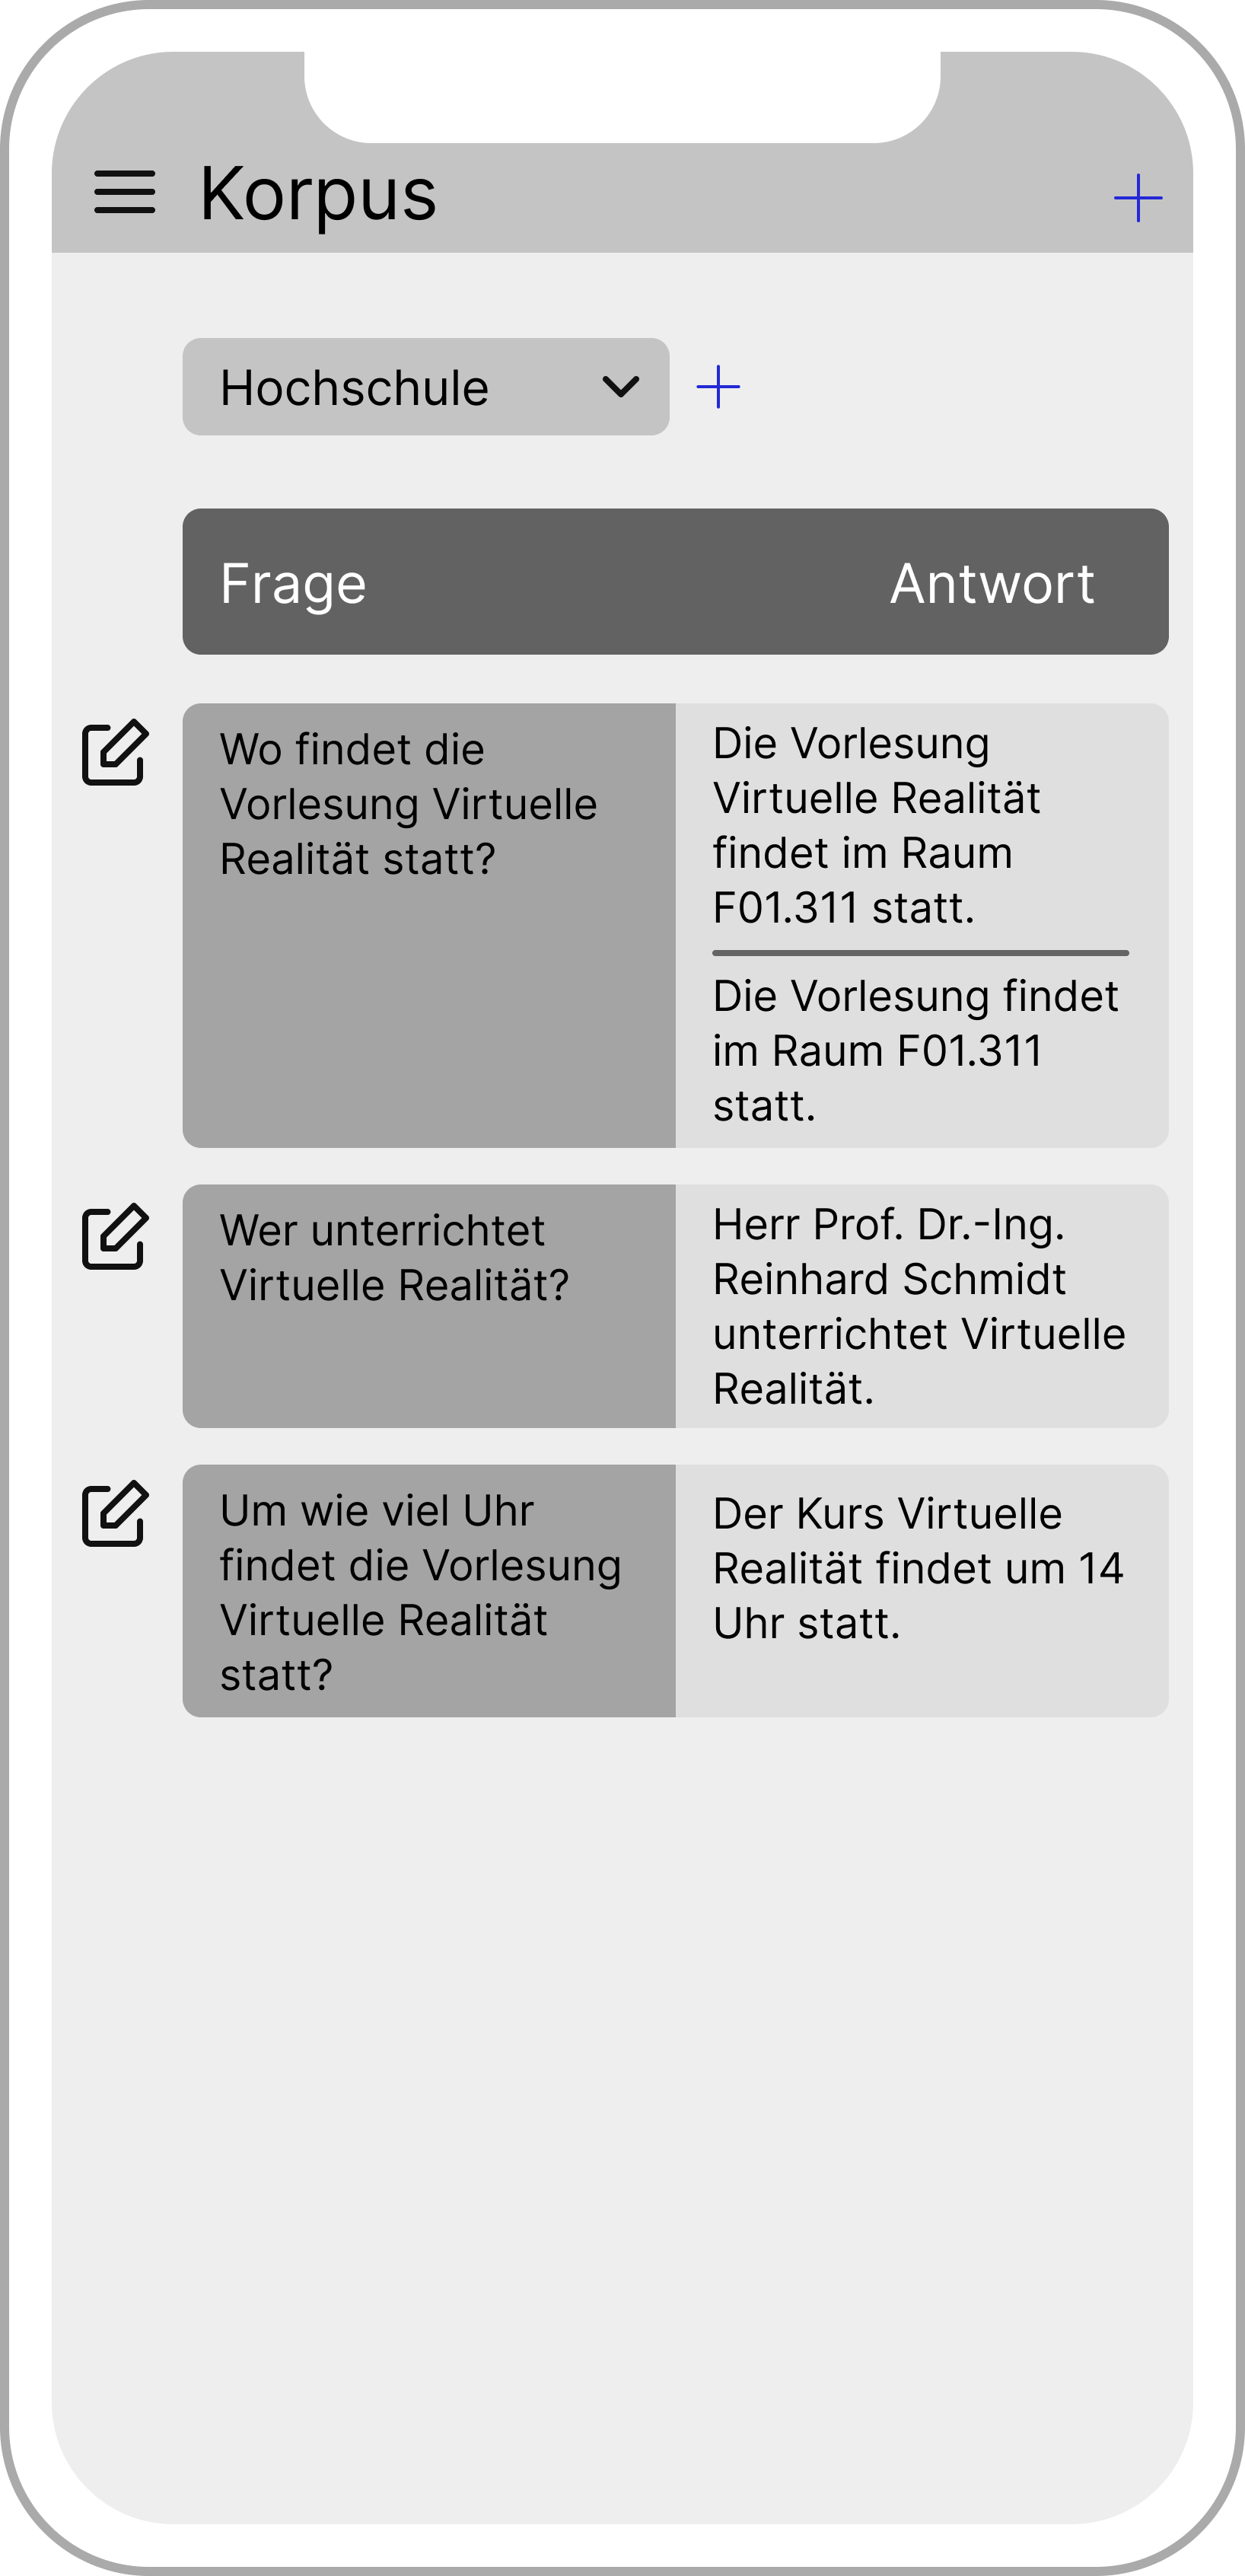
\includegraphics[width=0.5\textwidth]{bilder/new vers. UI Design/Korpus/iPhone X Korpus I.png}
    \caption{New version UI Design Admin-Interface Korpus mobile version}
    \label{fig:New version UI Design Admin-Interface Korpus mobile version}
\end{figure}
\noindent \textbf{Admin Webinterface mobil: Korpus} \newline
In der mobilen Version des Korpus kann man die Elemente genauso editieren wie im Webbrowser.

\newpage
\subsubsection{Version 2 Admin Interface Einstellungen}
Hier werden die neueren Versionen des UI Designs für das Admin-Interface Einstellungen vorgestellt.

\begin{figure}[H]
    \centering
    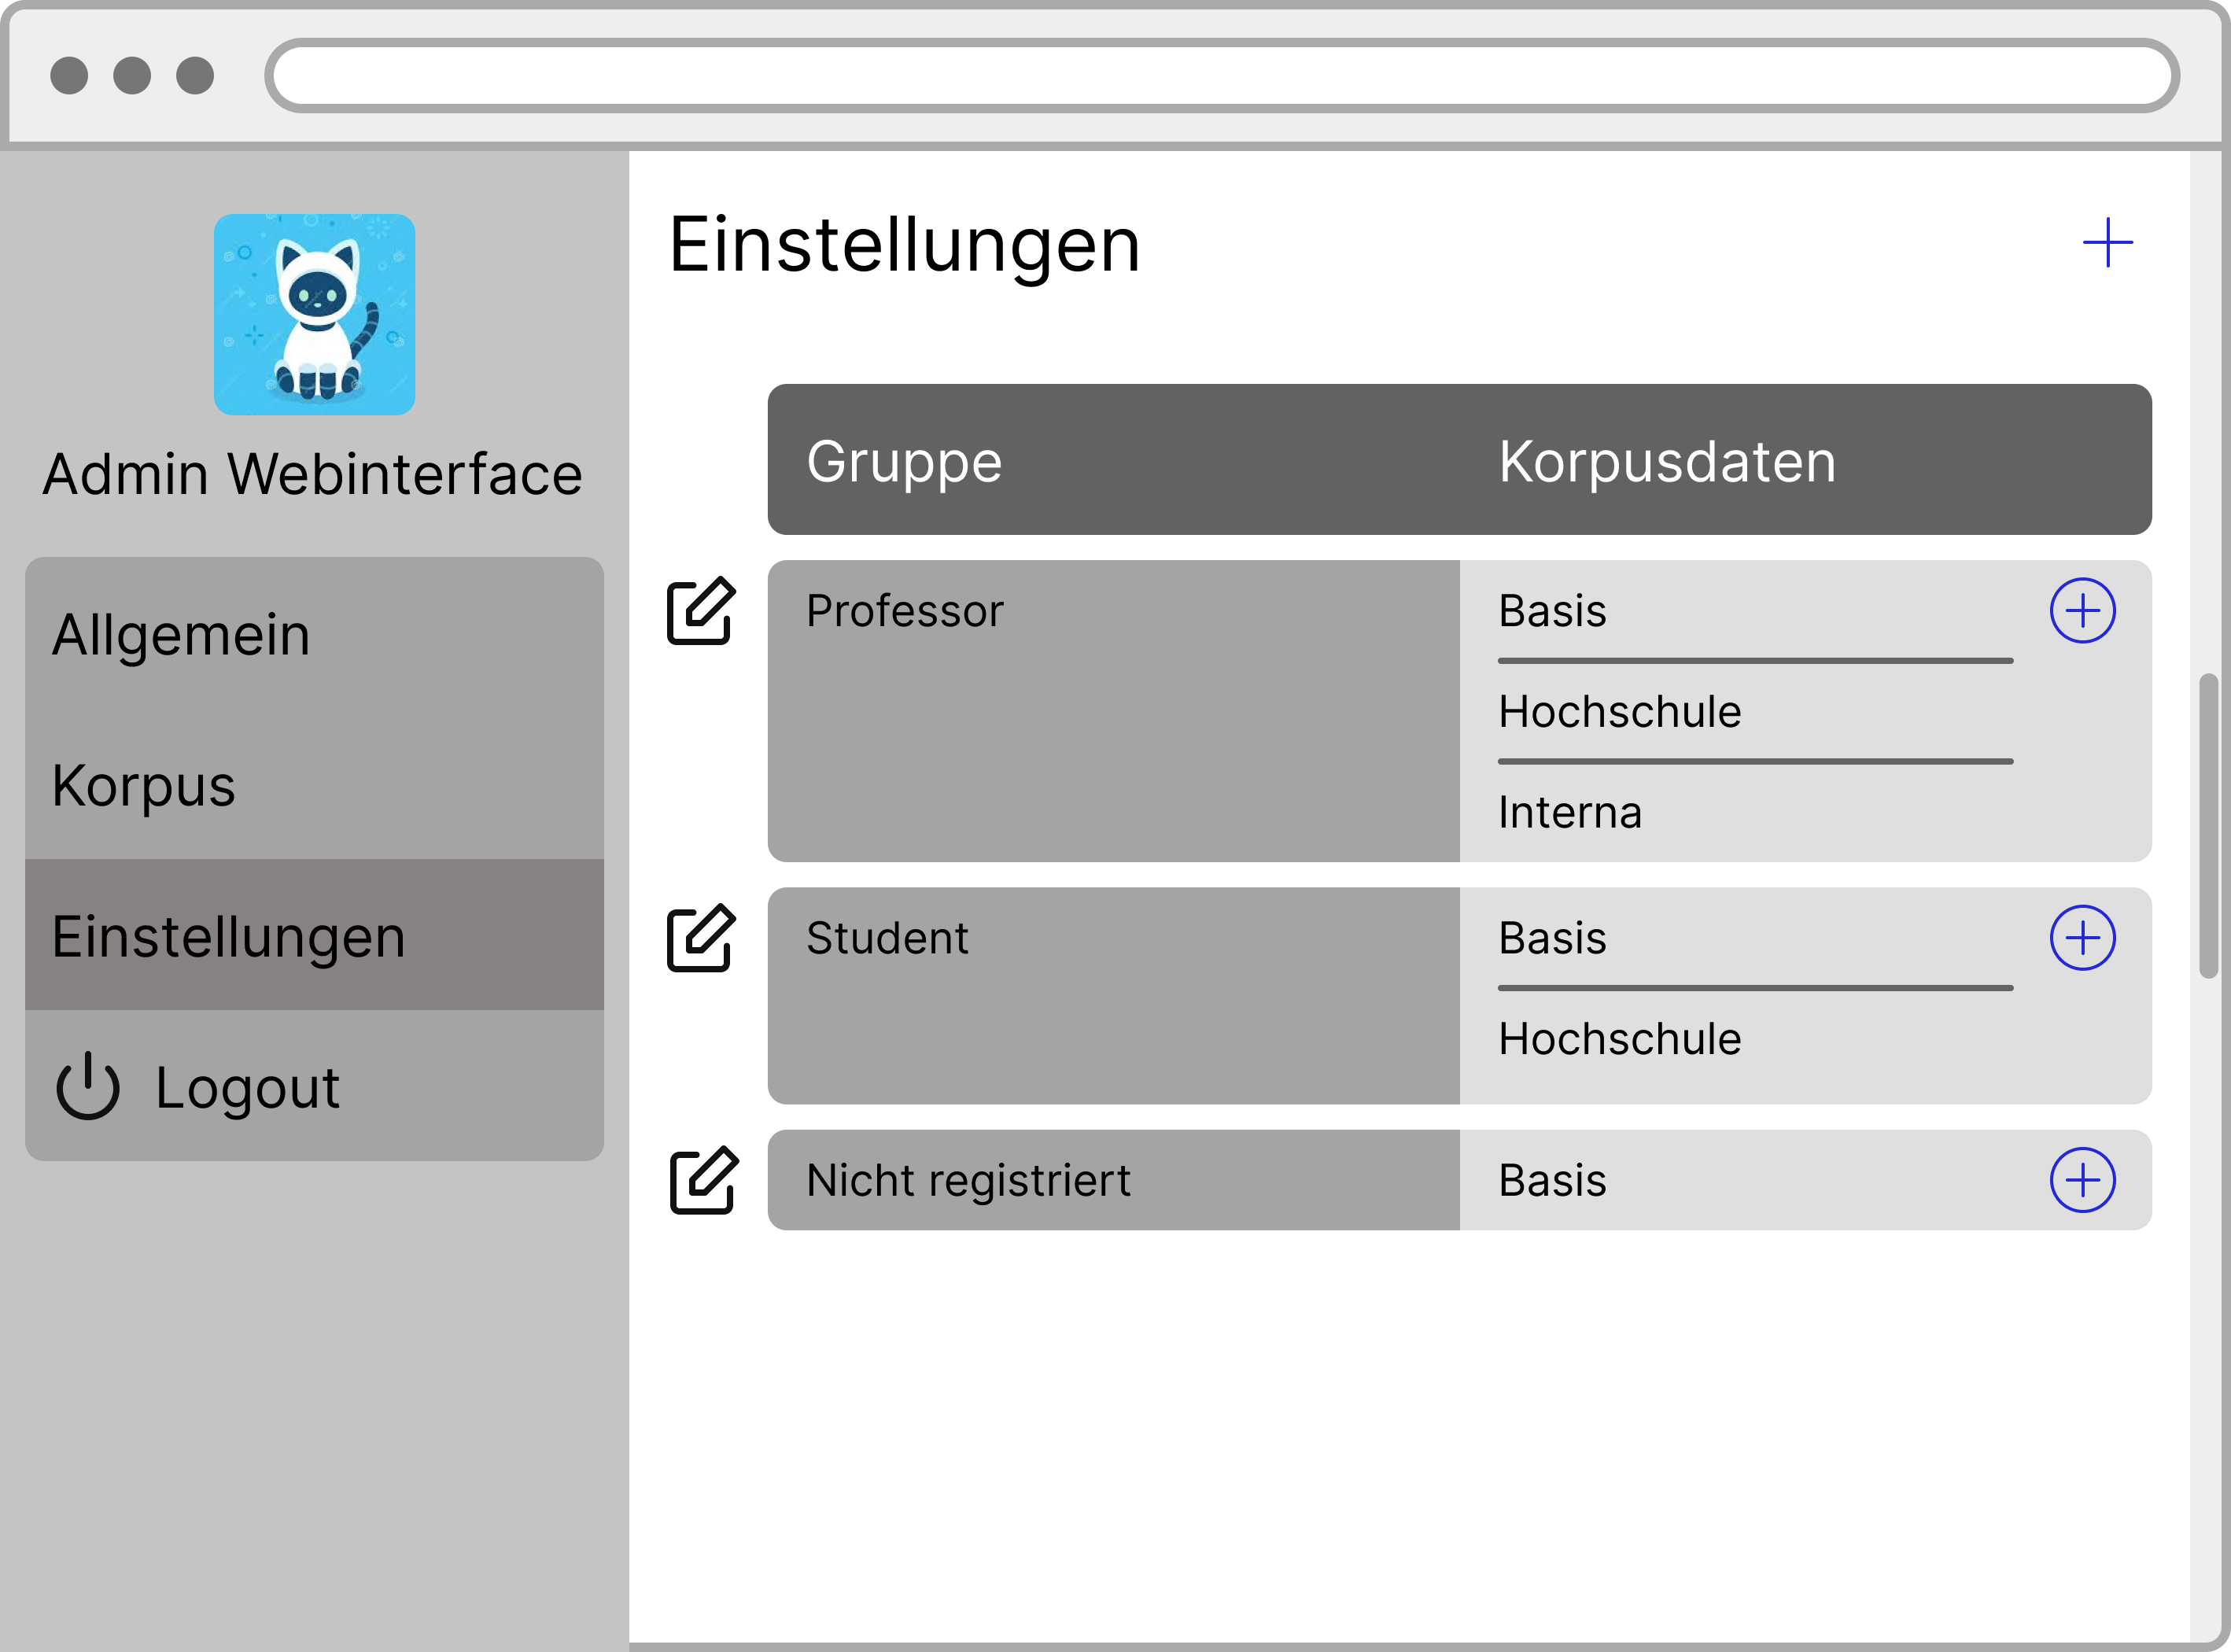
\includegraphics[width=1.0\textwidth]{bilder/new vers. UI Design/Einstellungen/Einstellungen (1).png}
    \caption{New version UI Design Admin-Interface Einstellungen}
    \label{fig:New version UI Design Admin-Interface Einstellungen}
\end{figure}
\noindent \textbf{Admin Webinterface: Einstellungen} \newline
In Einstellungen kann der Admin seine Gruppen einsehen, hinzufügen und entfernen. Er kann auch
die dazugehörenden Korpusdaten sehen und bearbeiten. In den Korpusdaten sind die Domänen der jeweiligen Gruppe eingetragen.

\begin{figure}[H]
    \centering
    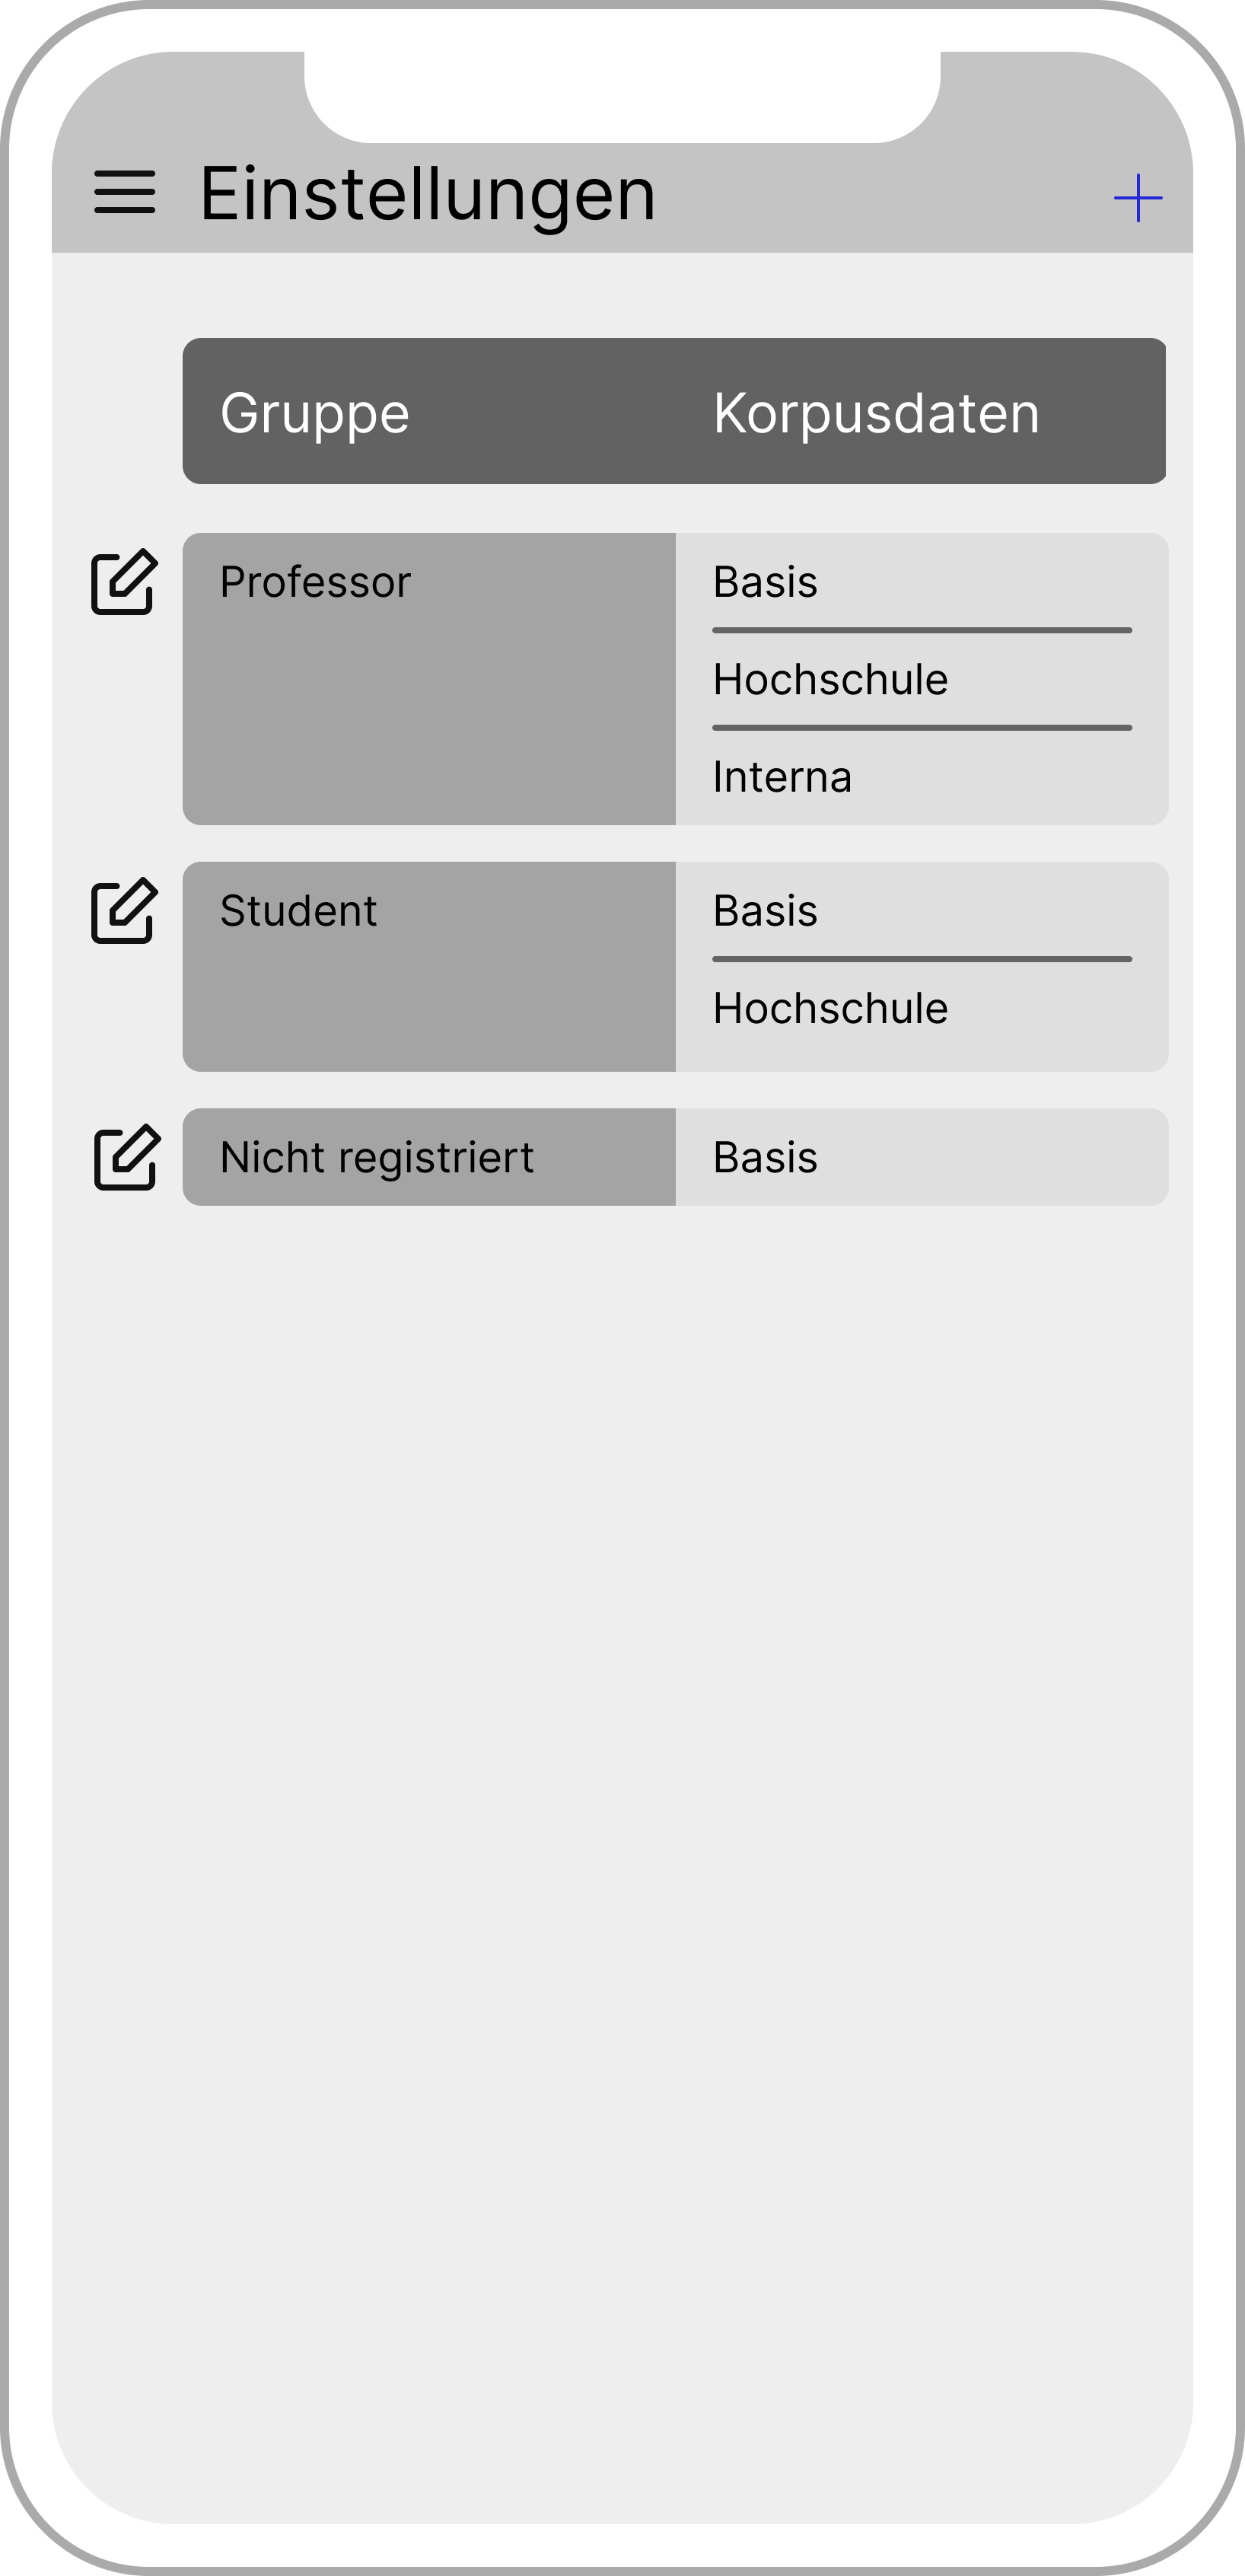
\includegraphics[width=0.5\textwidth]{bilder/new vers. UI Design/Einstellungen/iPhone X Einstellungen I (1).png}
    \caption{New version UI Design Admin-Interface Einstellungen mobile version}
    \label{fig:New version UI Design Admin-Interface Einstellungen mobile version}
\end{figure}
\noindent \textbf{Admin Webinterface mobil: Einstellungen} \newline
In der mobilen Version kann man ebenso die gleichen Features nutzen.

\newpage

\subsubsection{Version 2 Admin Interface Login}
Hier werden die neueren Versionen des UI Designs für das Admin-Interface Login vorgestellt.

\begin{figure}[H]
    \centering
    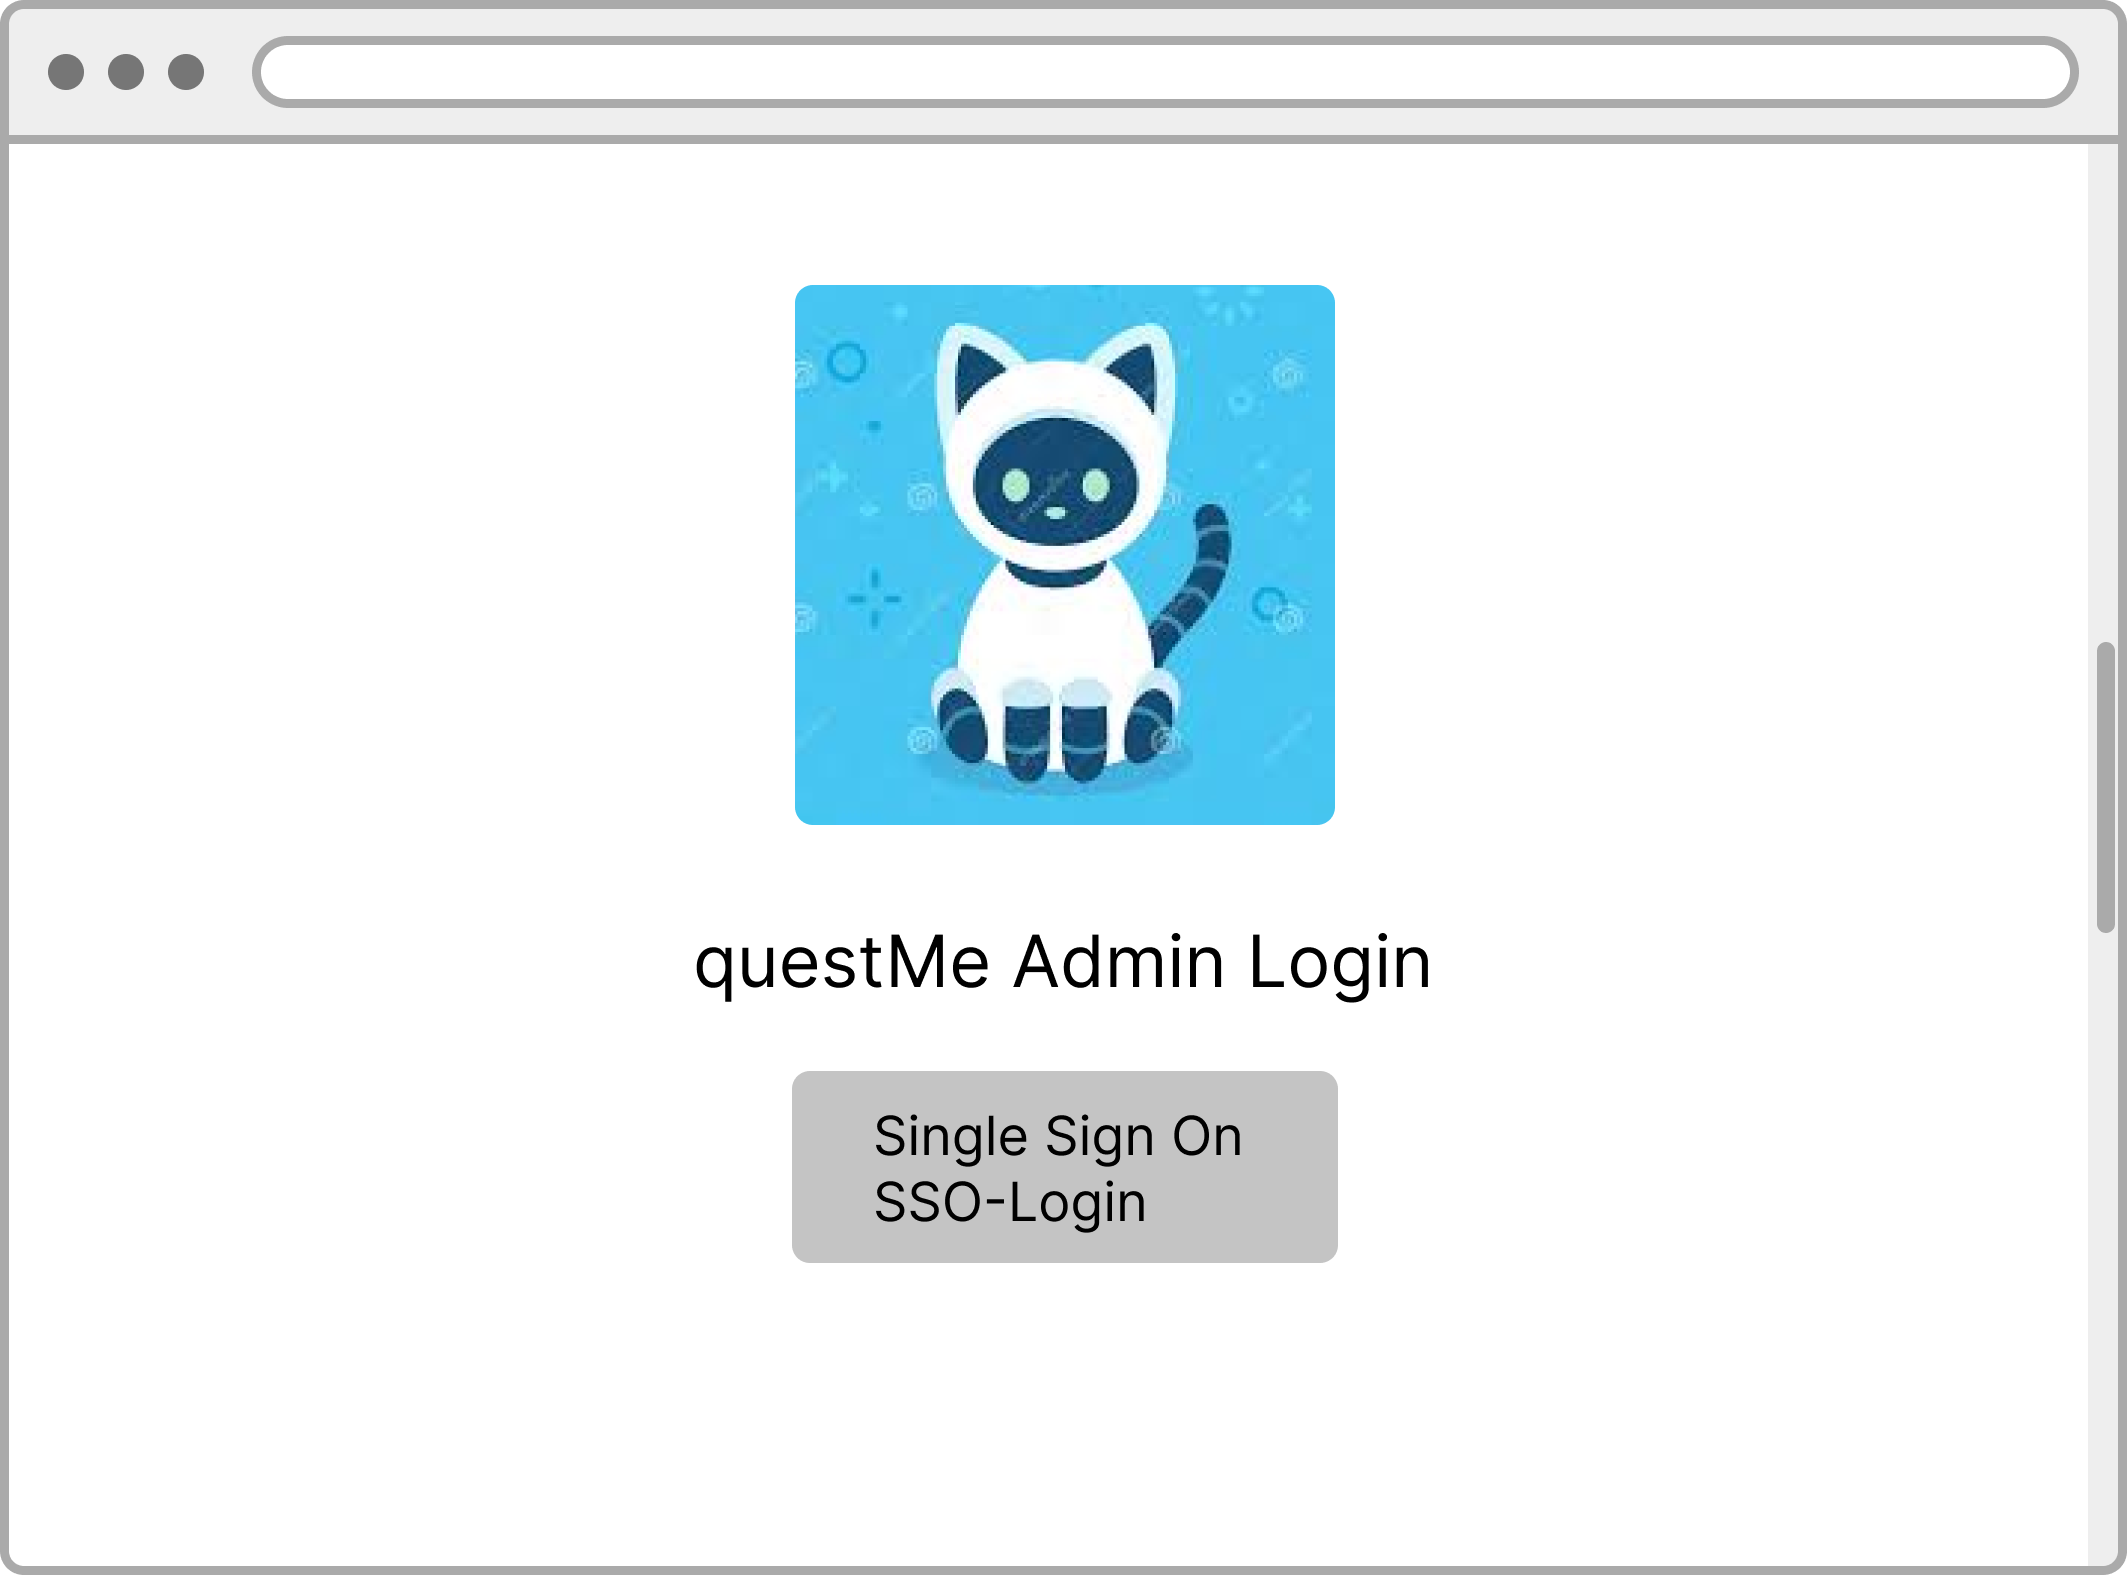
\includegraphics[width=1.0\textwidth]{bilder/new vers. UI Design/Login SSO/Admin Interface SSO.png}
    \caption{New version UI Design Admin-Interface Login}
    \label{fig:New version UI Design Admin-Interface Login}
\end{figure}
\noindent \textbf{Admin Webinterface: Single Sign On} \newline
Mit einem Link gelangt der Admin zu der Admin Login Seite, wo er mit Shibboleth sich einloggen kann. 

\begin{figure}[H]
    \centering
    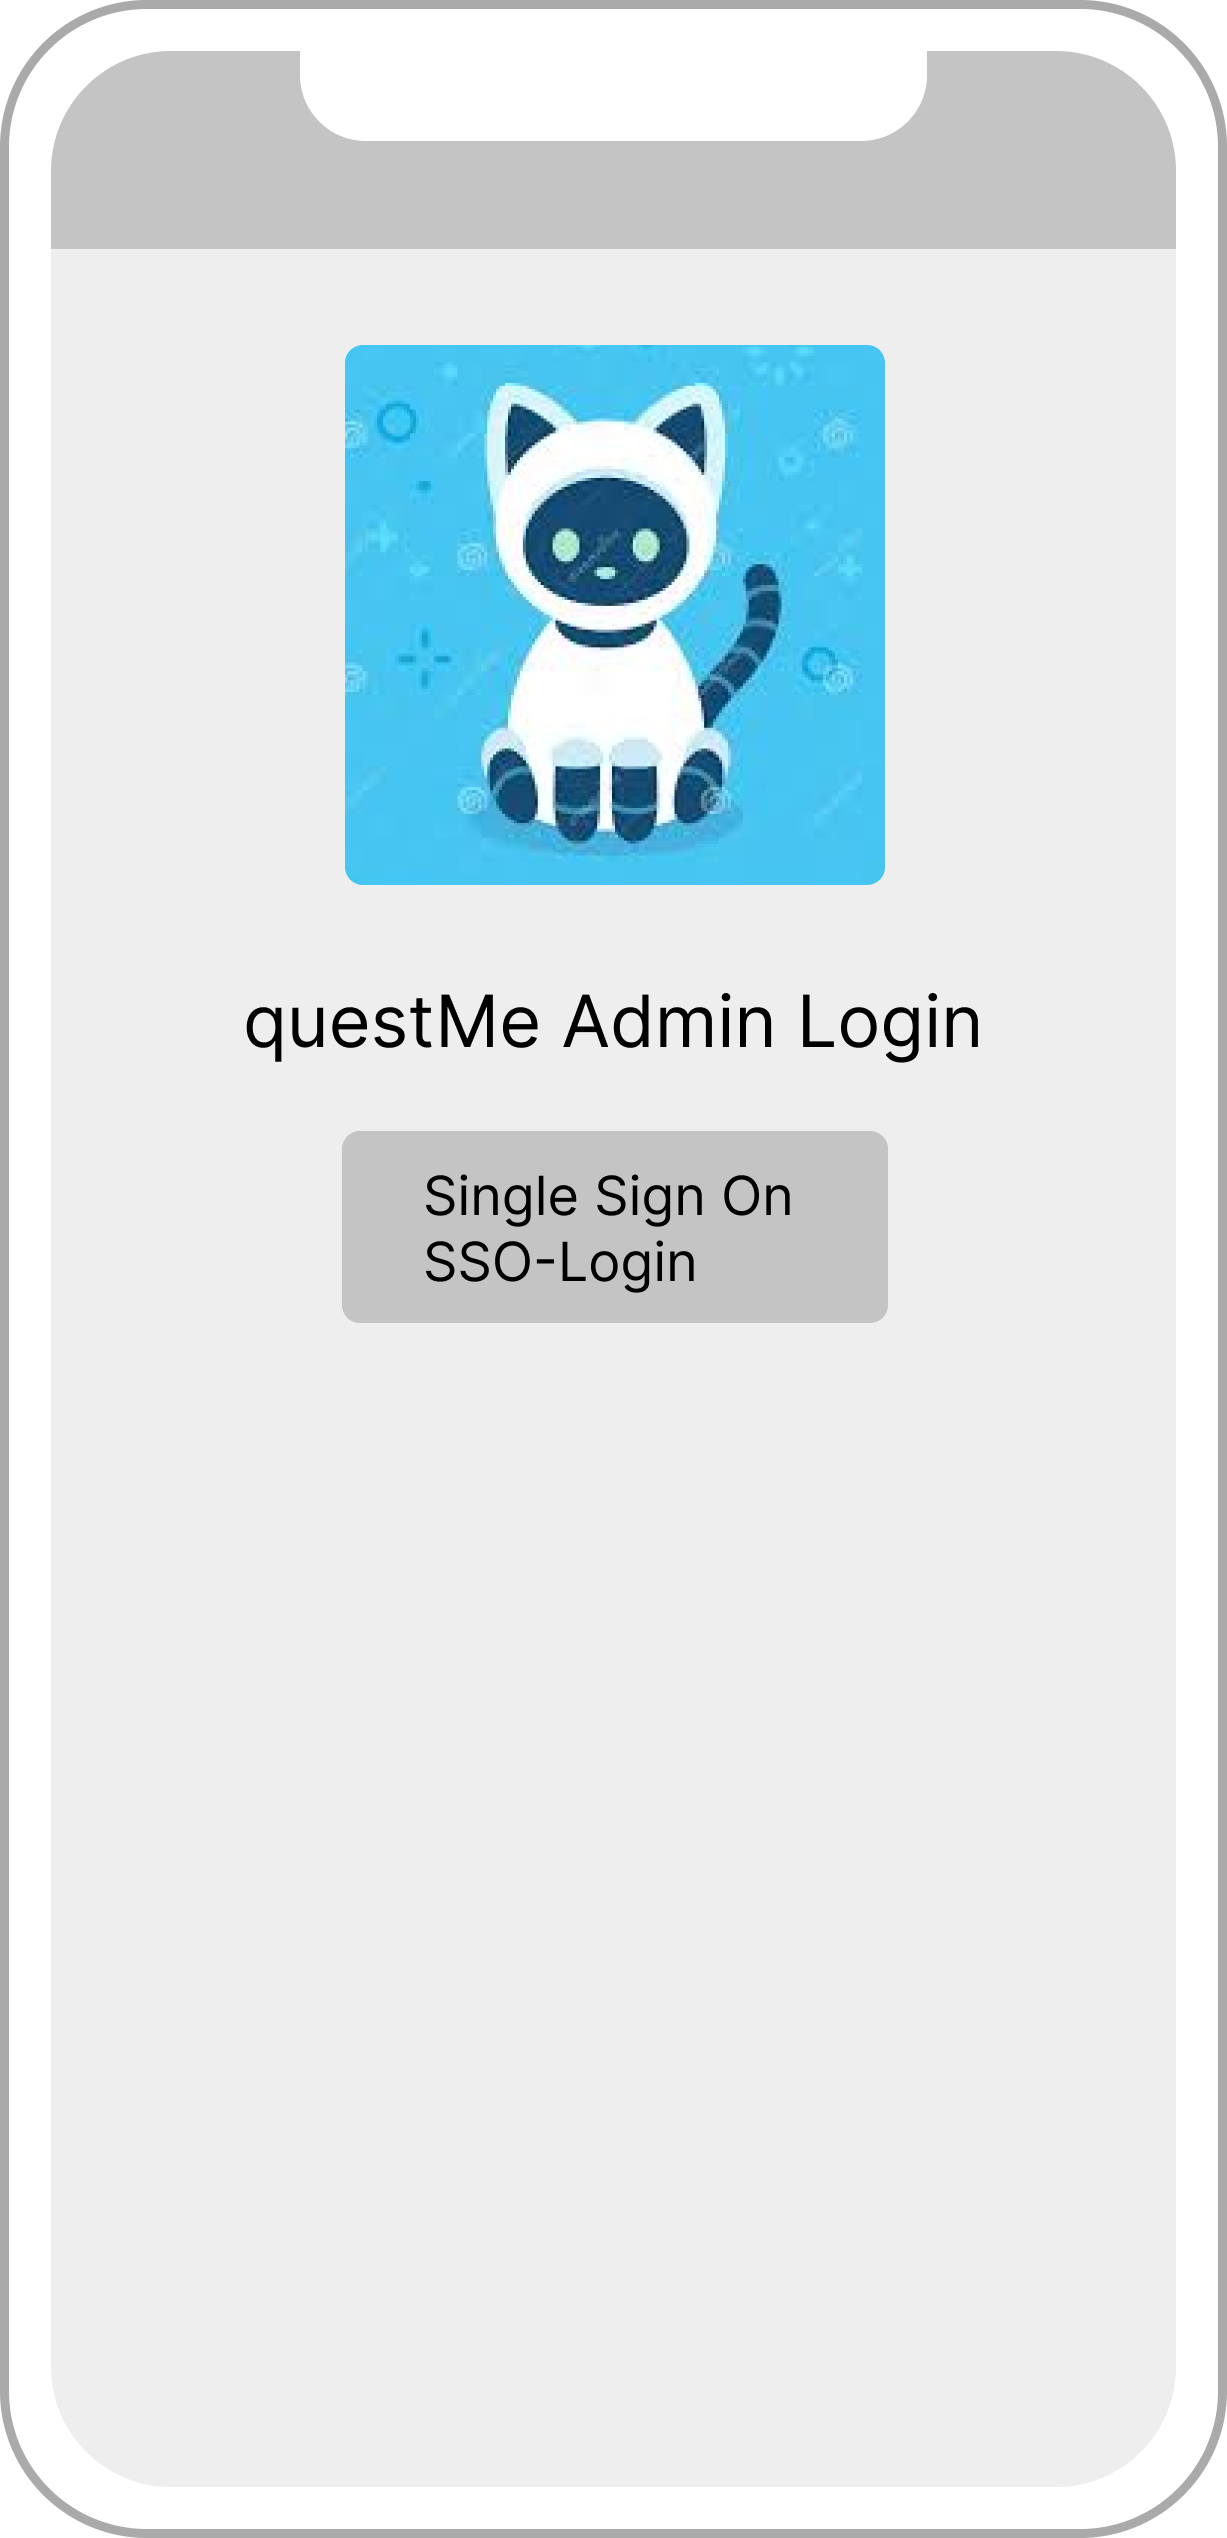
\includegraphics[width=0.5\textwidth]{bilder/new vers. UI Design/Login SSO/Interface SSO v1.2.png}
    \caption{New version UI Design Admin-Interface Login mobile version}
    \label{fig:New version UI Design Admin-Interface Login mobile version}
\end{figure}
\noindent \textbf{Admin Webinterface mobil: Single Sign On} \newline
In der mobilen Version wird die gleiche Prozedur benutzt.

\newpage

\subsection{Bisheriger Prototyp vom UI-Design}
Hier wird der bisherige Prototyp des UI-Designs, 
welche wir mit Angular bis jetzt programmiert haben, dargestellt.

\subsubsection{Prototyp Webchat}
Hier wird der Prototyp vom Webchat vorgestellt.

\begin{figure}[H]
    \centering
    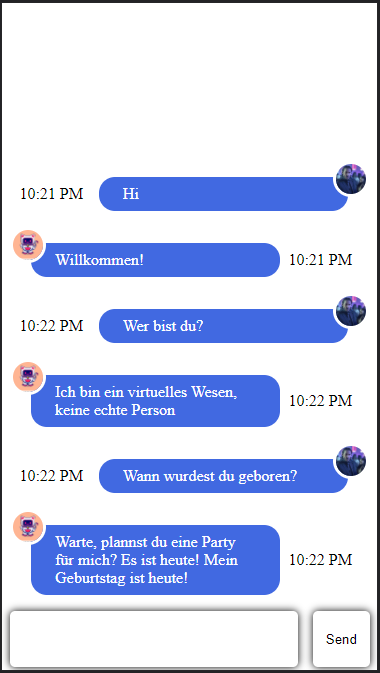
\includegraphics[width=0.5\textwidth]{bilder/prototyp UI Design/Chatinterface mobil.png}
    \caption{Prototyp Chat Interface}
    \label{fig:Prototyp Chat Interface}
\end{figure}
\noindent \textbf{Chat Interface} \newline
Dies ist der bisherige Prototyp des Chat Interfaces. Wie man hier sieht haben wir schon auf eine 
gute Lesbarkeit des Chats geachtet und auch mobile-first entwickelt.

\begin{figure}[H]
    \centering
    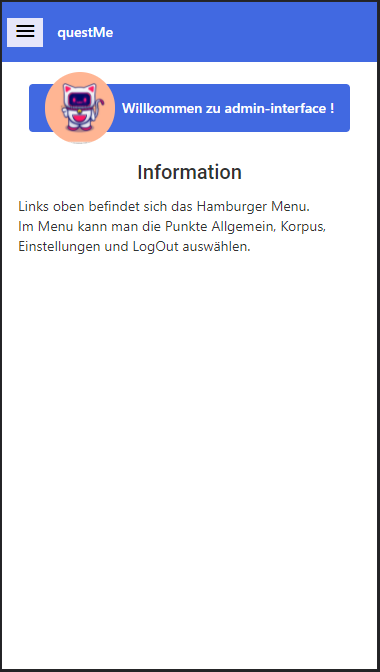
\includegraphics[width=0.5\textwidth]{bilder/prototyp UI Design/admininteface.png}
    \caption{Admin Interface Infoseite}
    \label{fig:Admin Interface Infoseite}
\end{figure}
\noindent \textbf{Admin Interface Infoseite} \newline
Hier haben wir die Admin Interface Infoseite, wo der Admin begrüßt wird.

\begin{figure}[H]
    \centering
    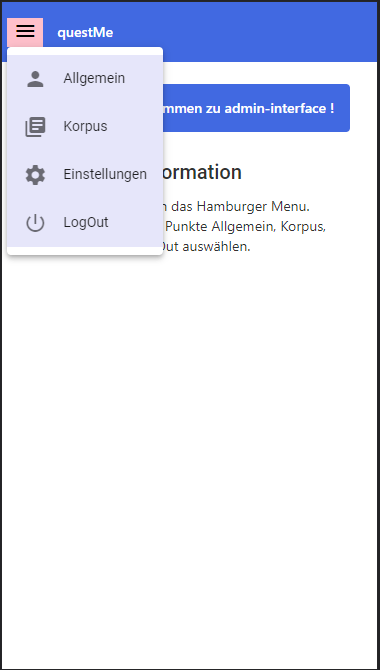
\includegraphics[width=0.5\textwidth]{bilder/prototyp UI Design/hamburgermenu_admininterface.png}
    \caption{Admin Interface Hamburgermenu}
    \label{fig:Admin Interface Hamburgermenu}
\end{figure}
\noindent \textbf{Admin Interface Infoseite} \newline
Hier sieht man das ausgeklappte Hamburgermenü auf der Infoseite.


